\chapter{Background}\label{sec:chapter2}

In this chapter the mathematical background that later chapters rely on is introduced.

\section{Signals on the Sphere}

\begin{figure}[htpb]
	\capstart{}
	\subfloat[\(\pixel{Y_{00}}\)]
	{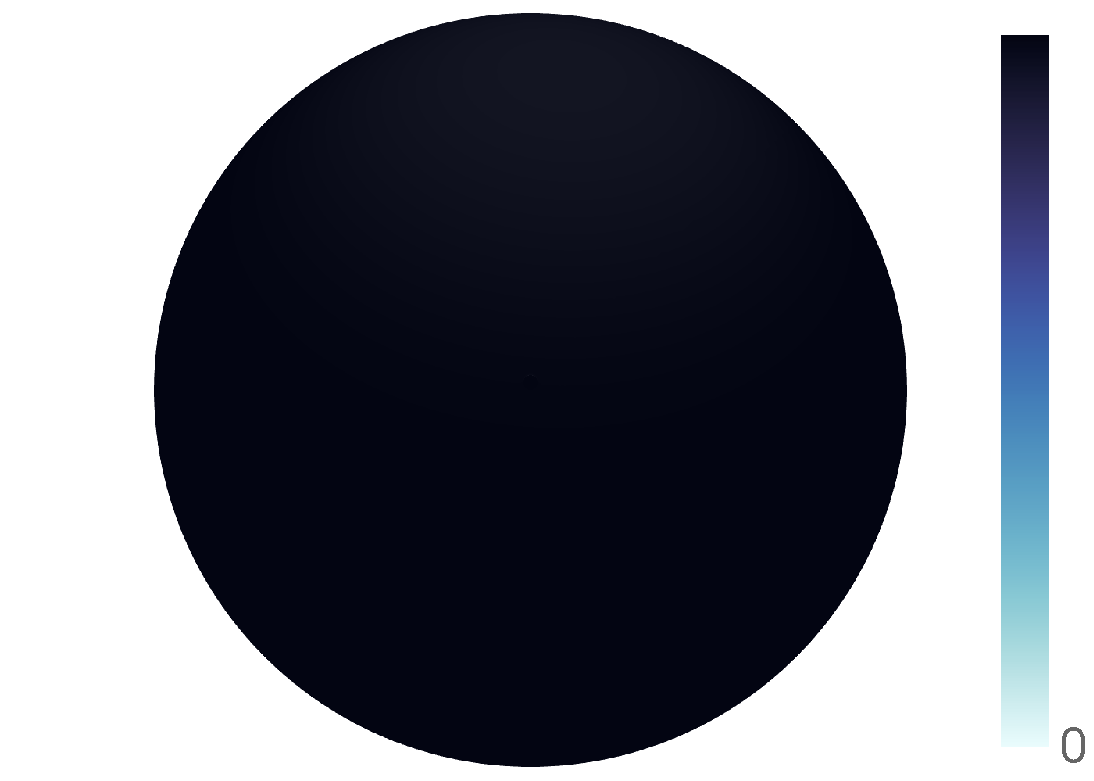
\includegraphics[trim={23 7 3 6},clip,width=.2\textwidth]{spherical_harmonic_0l_0m_L128_real_norm.pdf}}
	\newline
	\subfloat[\(\pixel{Y_{10}}\)]
	{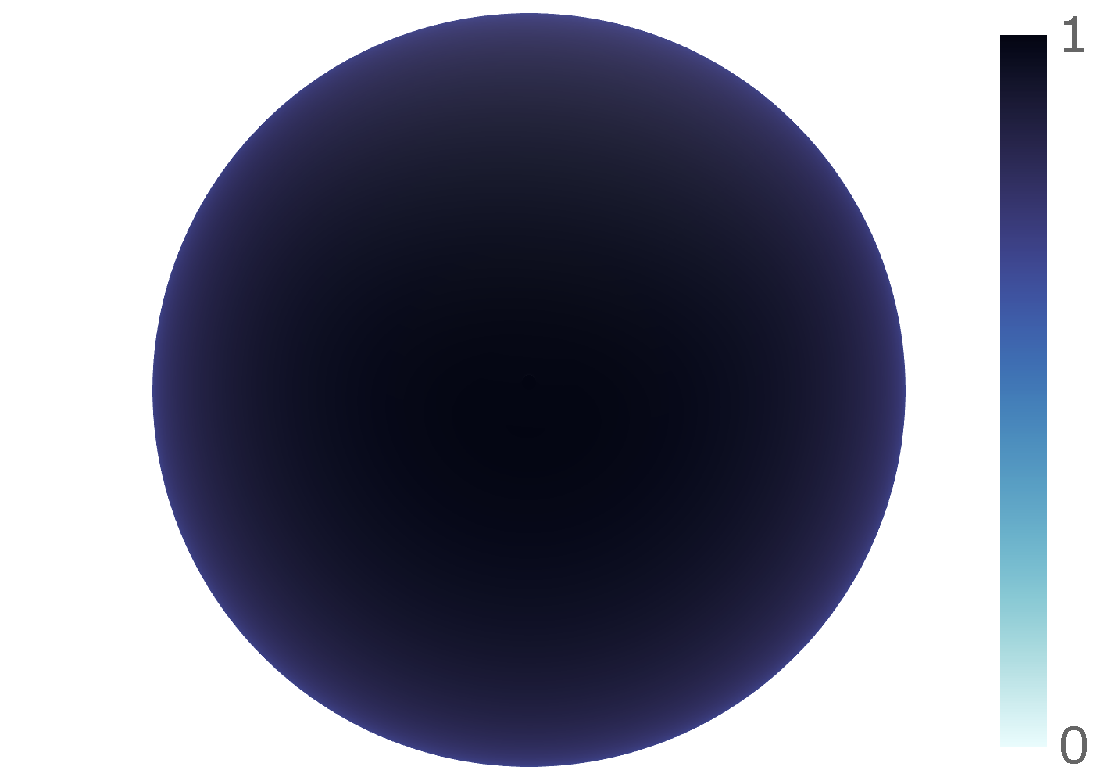
\includegraphics[trim={23 7 3 6},clip,width=.2\textwidth]{spherical_harmonic_1l_0m_L128_real_norm.pdf}}
	%
	\subfloat[\(\pixel{Y_{11}}\)]
	{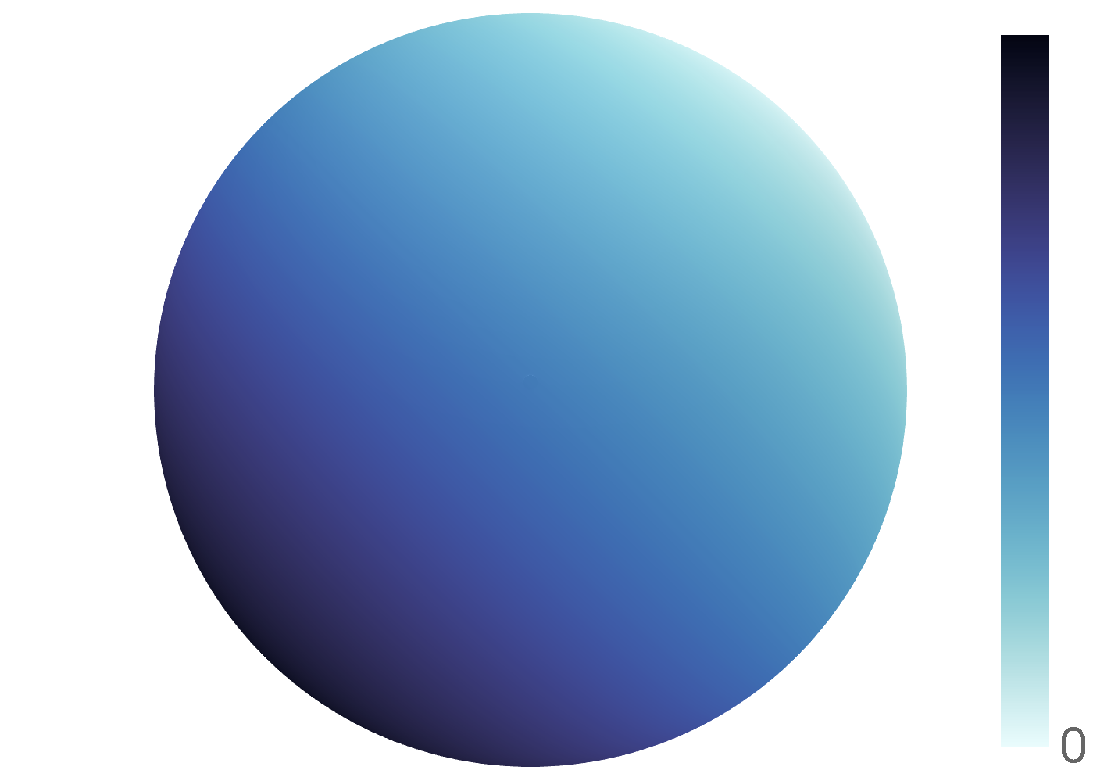
\includegraphics[trim={23 7 3 6},clip,width=.2\textwidth]{spherical_harmonic_1l_1m_L128_real_norm.pdf}}
	\newline
	\subfloat[\(\pixel{Y_{20}}\)]
	{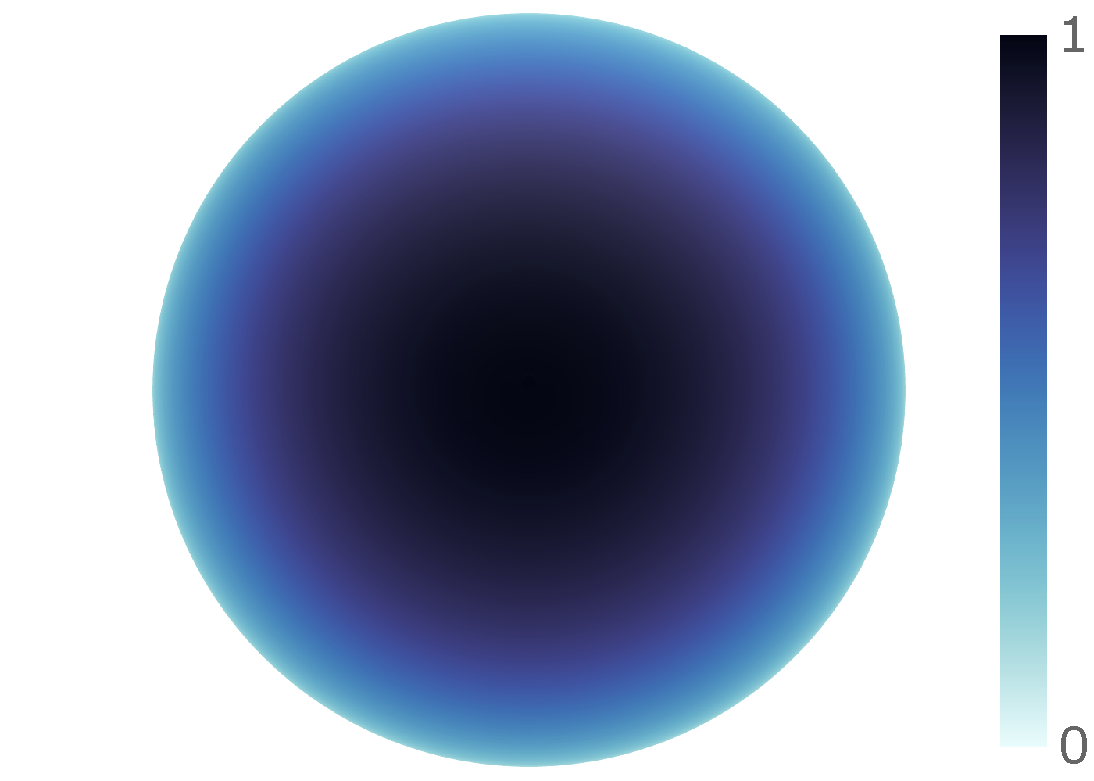
\includegraphics[trim={23 7 3 6},clip,width=.2\textwidth]{spherical_harmonic_2l_0m_L128_real_norm.pdf}}
	%
	\subfloat[\(\pixel{Y_{21}}\)]
	{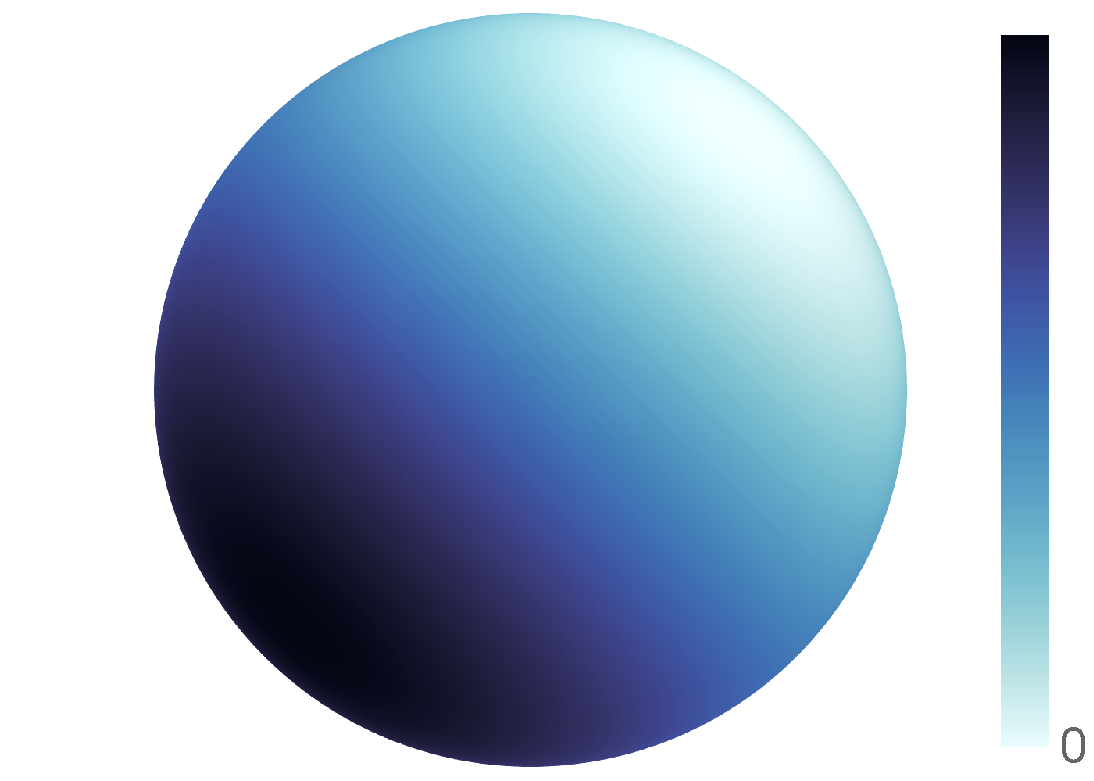
\includegraphics[trim={23 7 3 6},clip,width=.2\textwidth]{spherical_harmonic_2l_1m_L128_real_norm.pdf}}
	%
	\subfloat[\(\pixel{Y_{22}}\)]
	{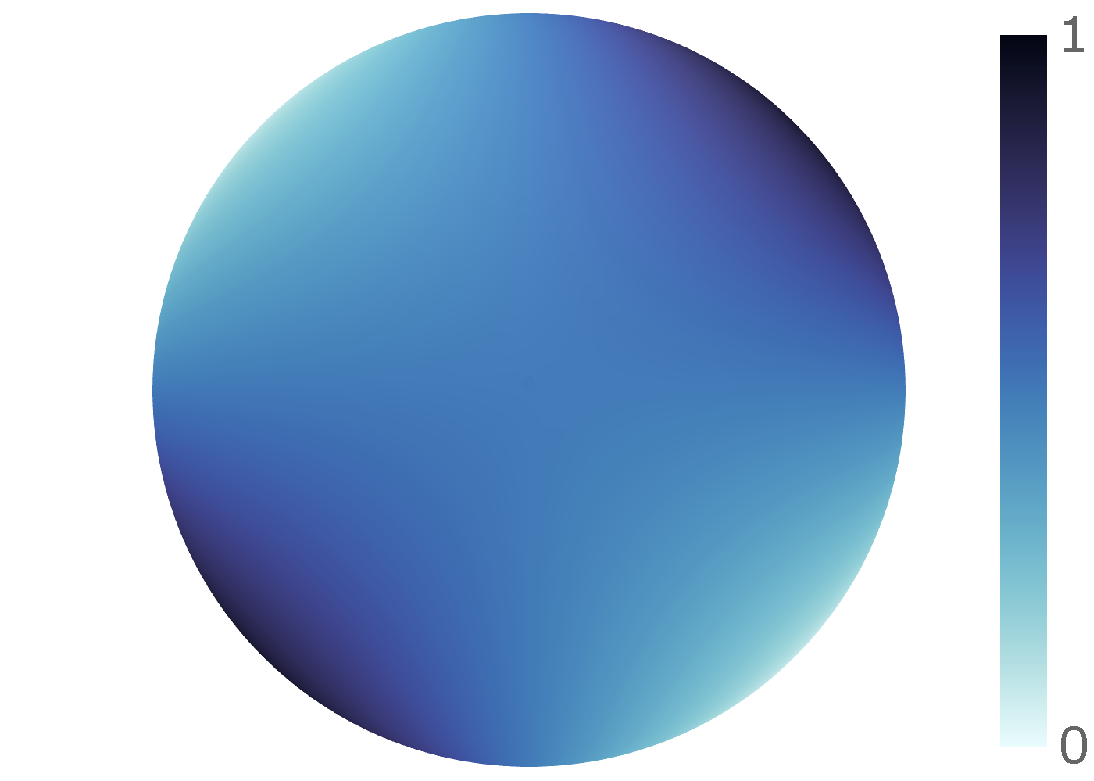
\includegraphics[trim={23 7 3 6},clip,width=.2\textwidth]{spherical_harmonic_2l_2m_L128_real_norm.pdf}}
	\newline
	\subfloat[\(\pixel{Y_{30}}\)]
	{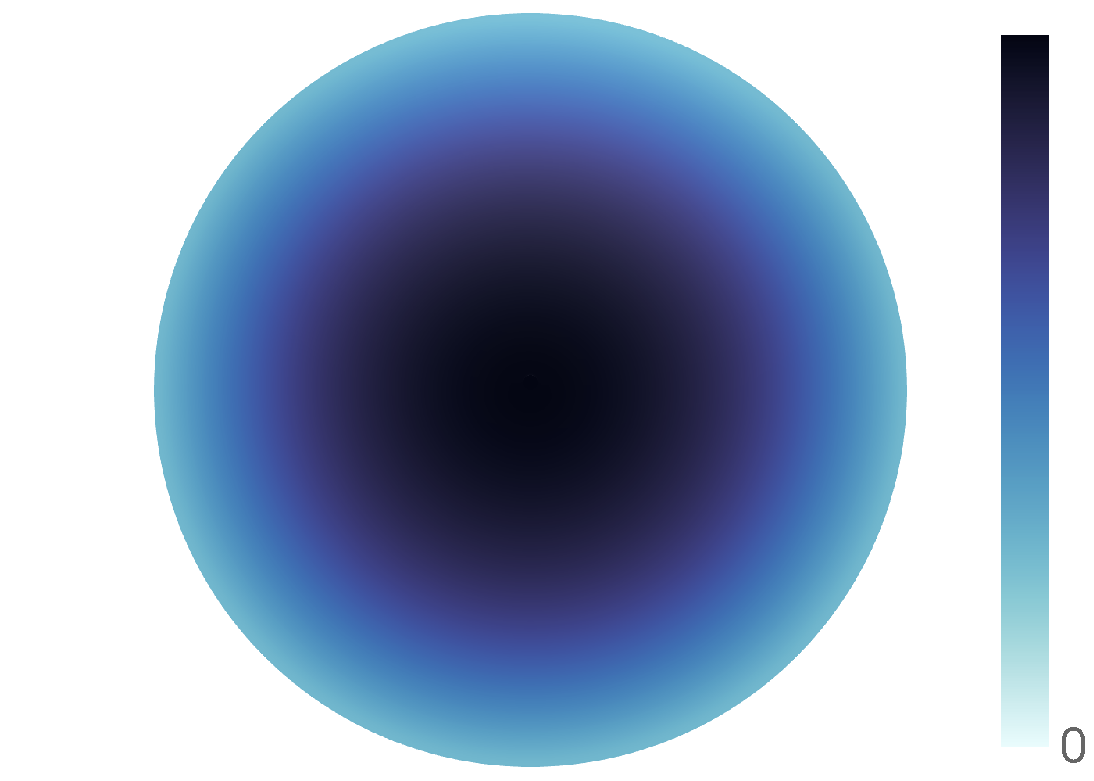
\includegraphics[trim={23 7 3 6},clip,width=.2\textwidth]{spherical_harmonic_3l_0m_L128_real_norm.pdf}}
	%
	\subfloat[\(\pixel{Y_{31}}\)]
	{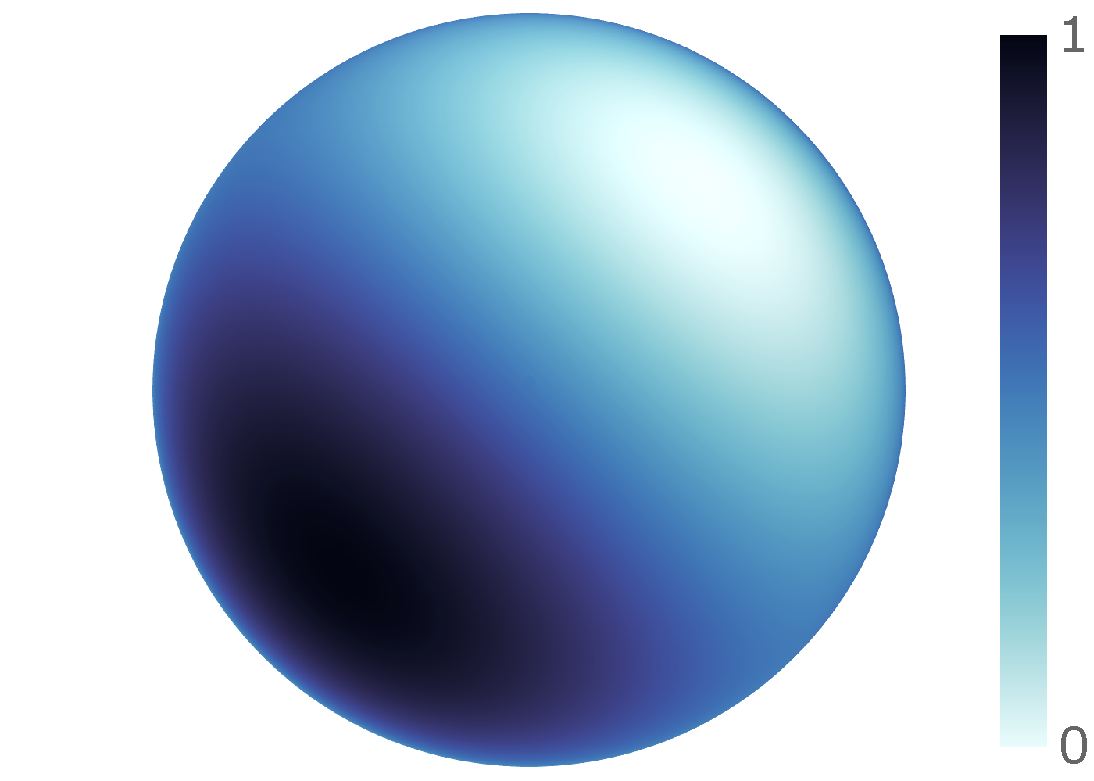
\includegraphics[trim={23 7 3 6},clip,width=.2\textwidth]{spherical_harmonic_3l_1m_L128_real_norm.pdf}}
	%
	\subfloat[\(\pixel{Y_{32}}\)]
	{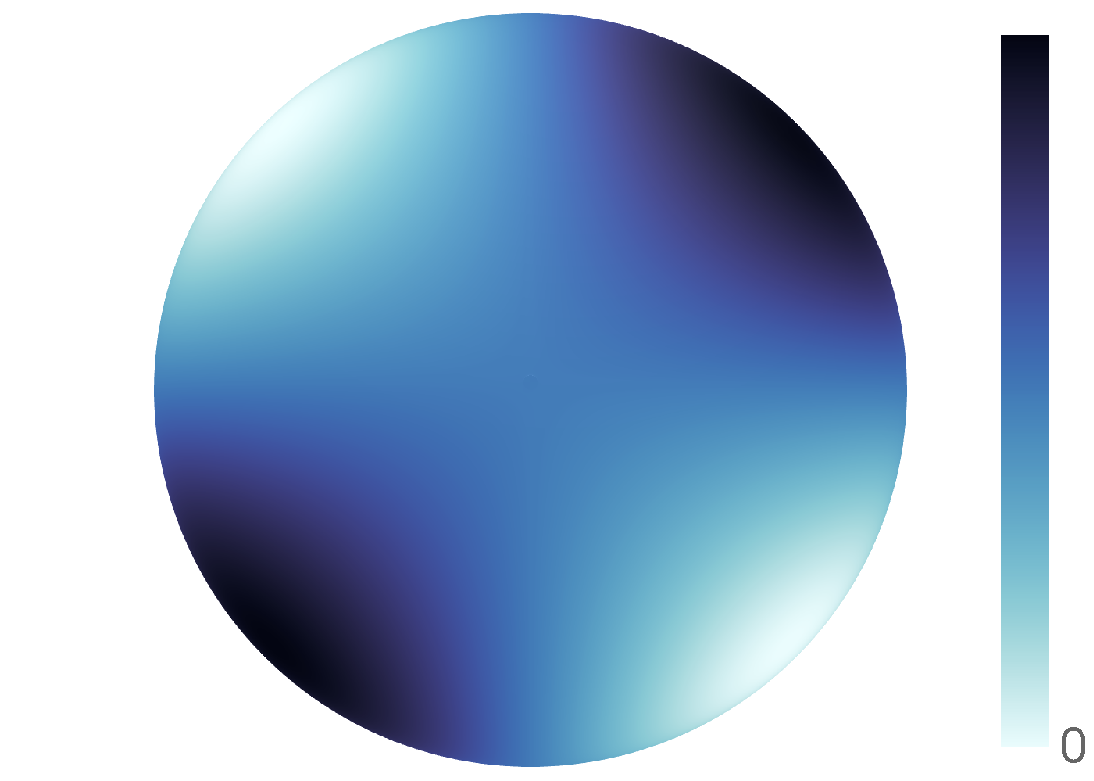
\includegraphics[trim={23 7 3 6},clip,width=.2\textwidth]{spherical_harmonic_3l_2m_L128_real_norm.pdf}}
	%
	\subfloat[\(\pixel{Y_{33}}\)]
	{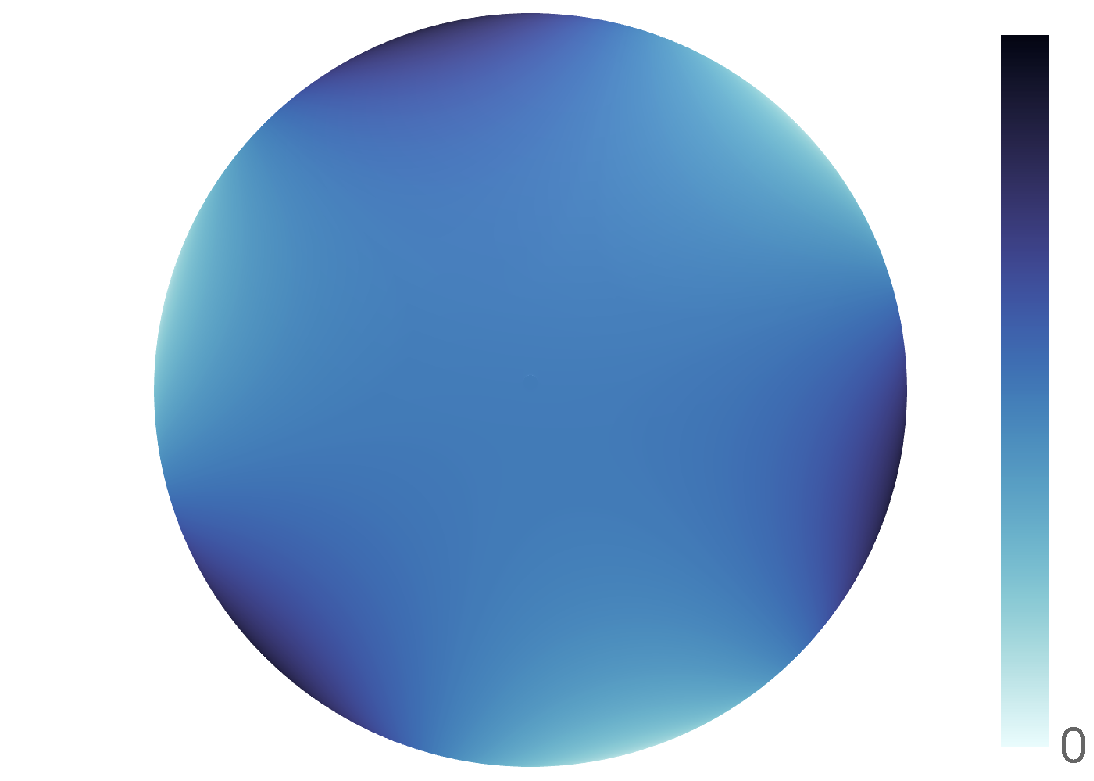
\includegraphics[trim={23 7 3 6},clip,width=.2\textwidth]{spherical_harmonic_3l_3m_L128_real_norm.pdf}}
	\newline
	\subfloat[\(\pixel{Y_{40}}\)]
	{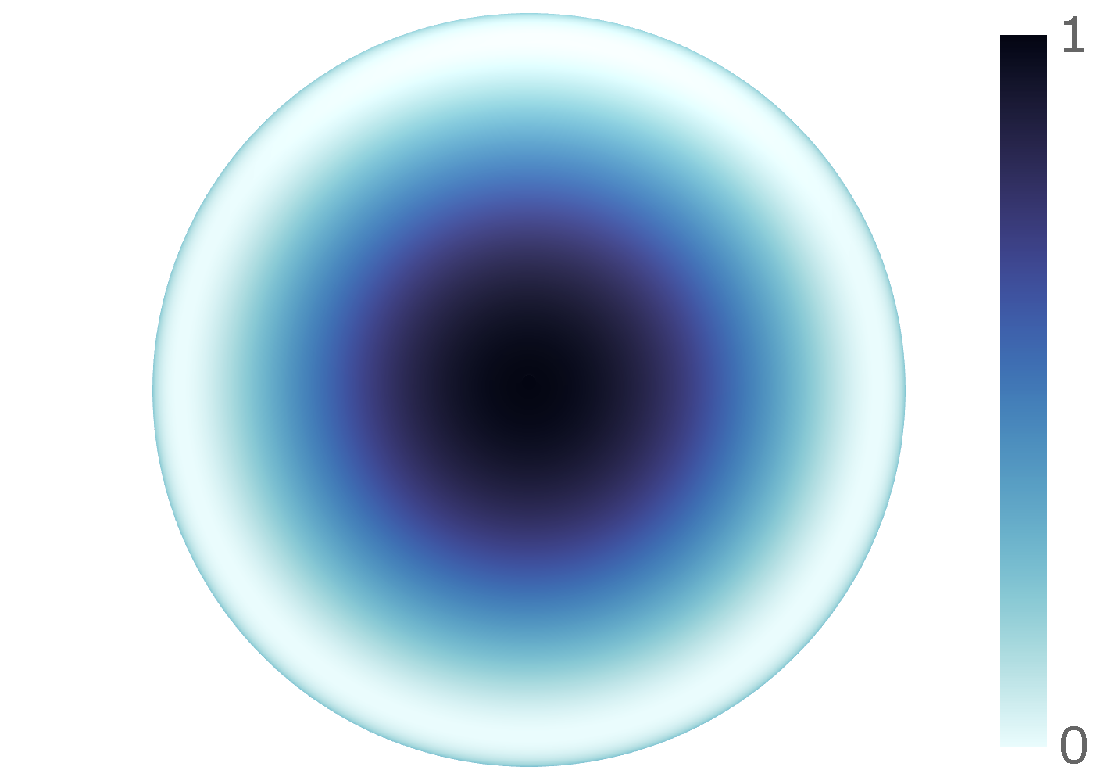
\includegraphics[trim={23 7 3 6},clip,width=.2\textwidth]{spherical_harmonic_4l_0m_L128_real_norm.pdf}}
	%
	\subfloat[\(\pixel{Y_{41}}\)]
	{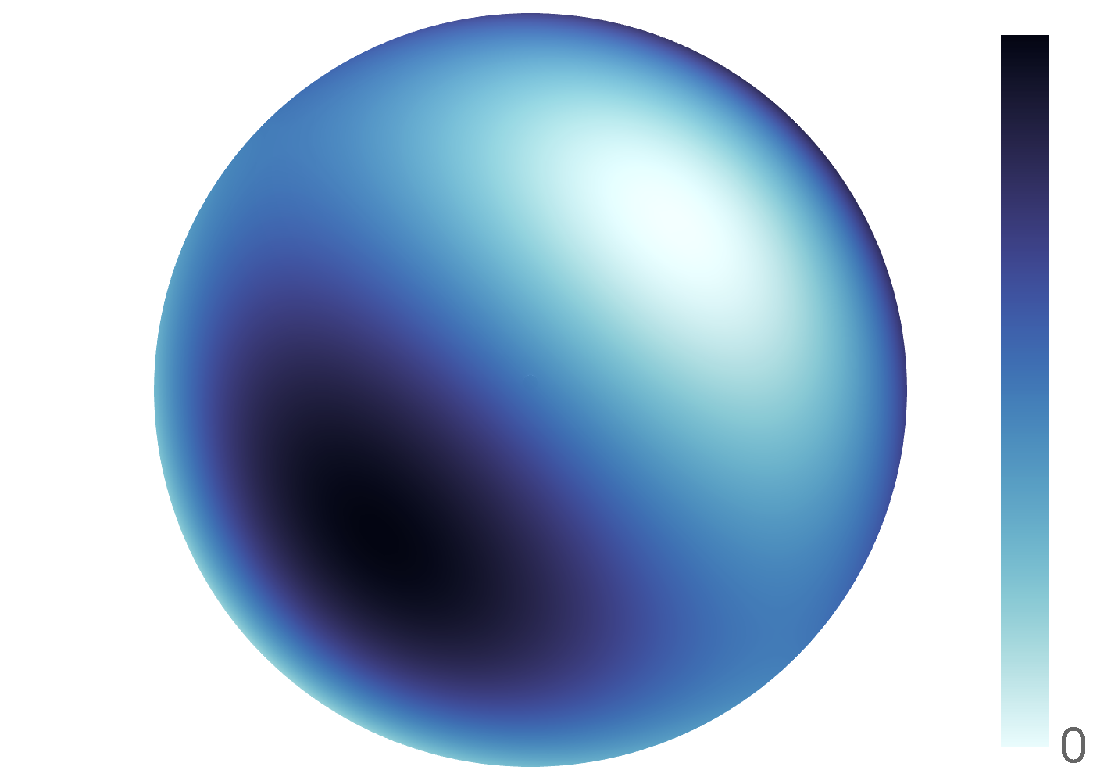
\includegraphics[trim={23 7 3 6},clip,width=.2\textwidth]{spherical_harmonic_4l_1m_L128_real_norm.pdf}}
	%
	\subfloat[\(\pixel{Y_{42}}\)]
	{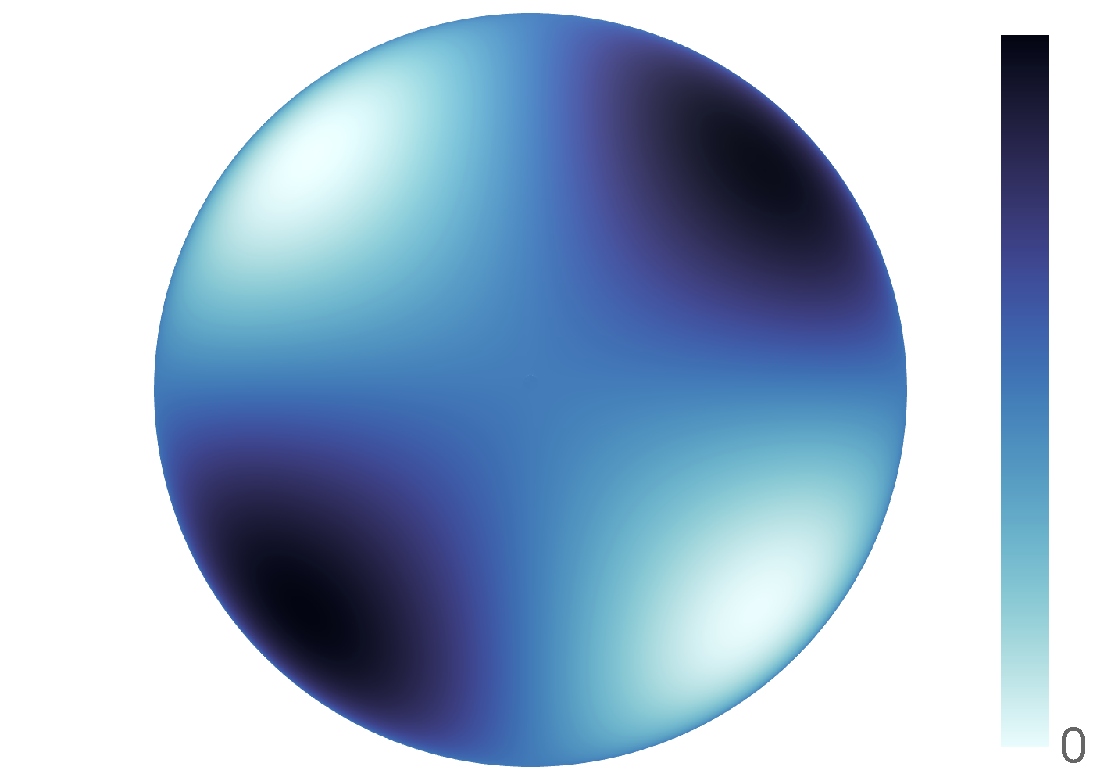
\includegraphics[trim={23 7 3 6},clip,width=.2\textwidth]{spherical_harmonic_4l_2m_L128_real_norm.pdf}}
	%
	\subfloat[\(\pixel{Y_{43}}\)]
	{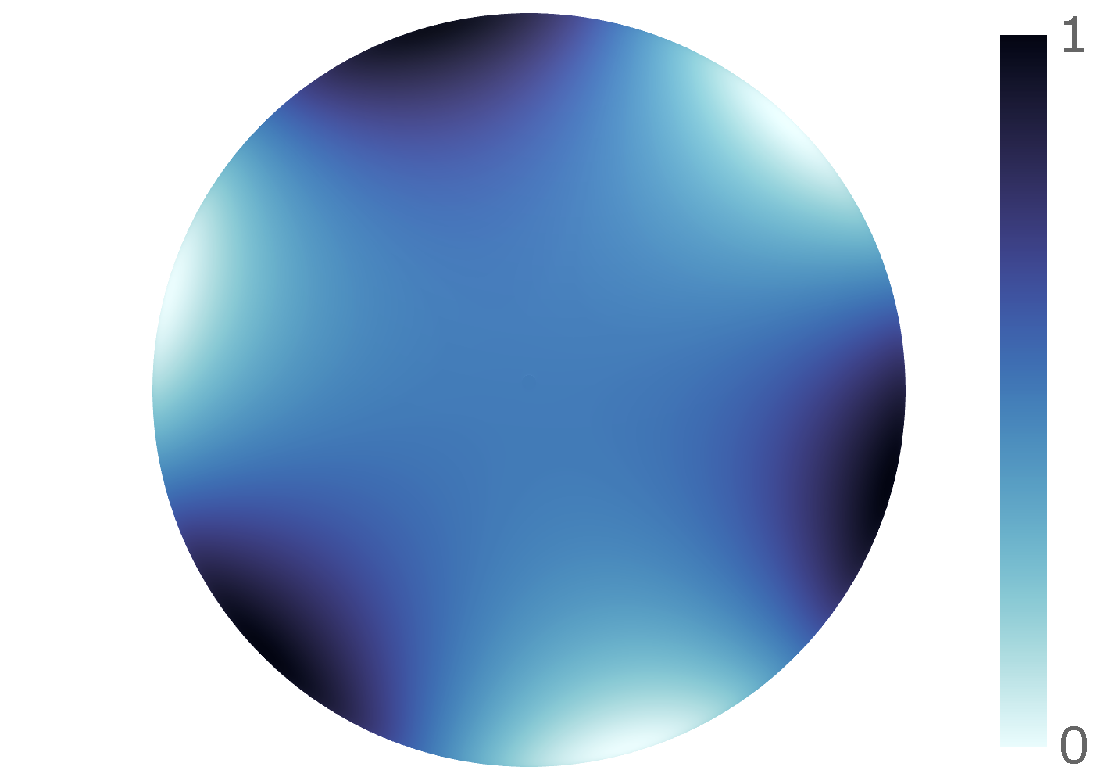
\includegraphics[trim={23 7 3 6},clip,width=.2\textwidth]{spherical_harmonic_4l_3m_L128_real_norm.pdf}}
	%
	\subfloat[\(\pixel{Y_{44}}\)]
	{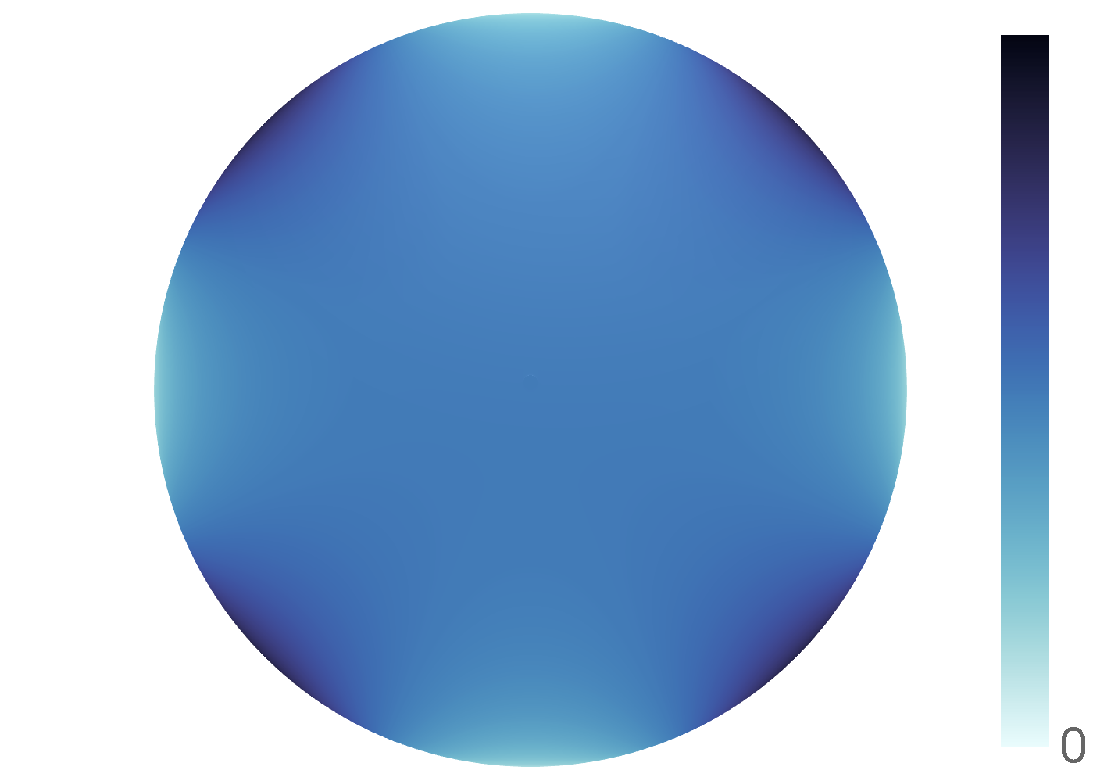
\includegraphics[trim={23 7 3 6},clip,width=.2\textwidth]{spherical_harmonic_4l_4m_L128_real_norm.pdf}}
	\caption[
		The spherical harmonics for \(\ell=0,\ldots,4\)
	]{
		The real part of the spherical harmonics \(\pixel{\harmonic{Y}}\) for \(\ell=0,\ldots,4\) (top-to-bottom) and \(m=0,\ldots,\ell{}\) (left-to-right).
		The negative order harmonics \(\pixel{Y_{\ell(-m)}}\) have not been included as they are simply rotated with respect to the positive order harmonics by \(\SI{90}{\degree}/m\).
	}\label{fig:chapter2_spherical_harmonics}
\end{figure}


\section{Wavelets}

\subsection{Euclidean}

\subsection{Sphere}

\begin{figure}[htpb]
	\centering\capstart{}
	\subfloat[\(\pixel{\Phi}\)]
	{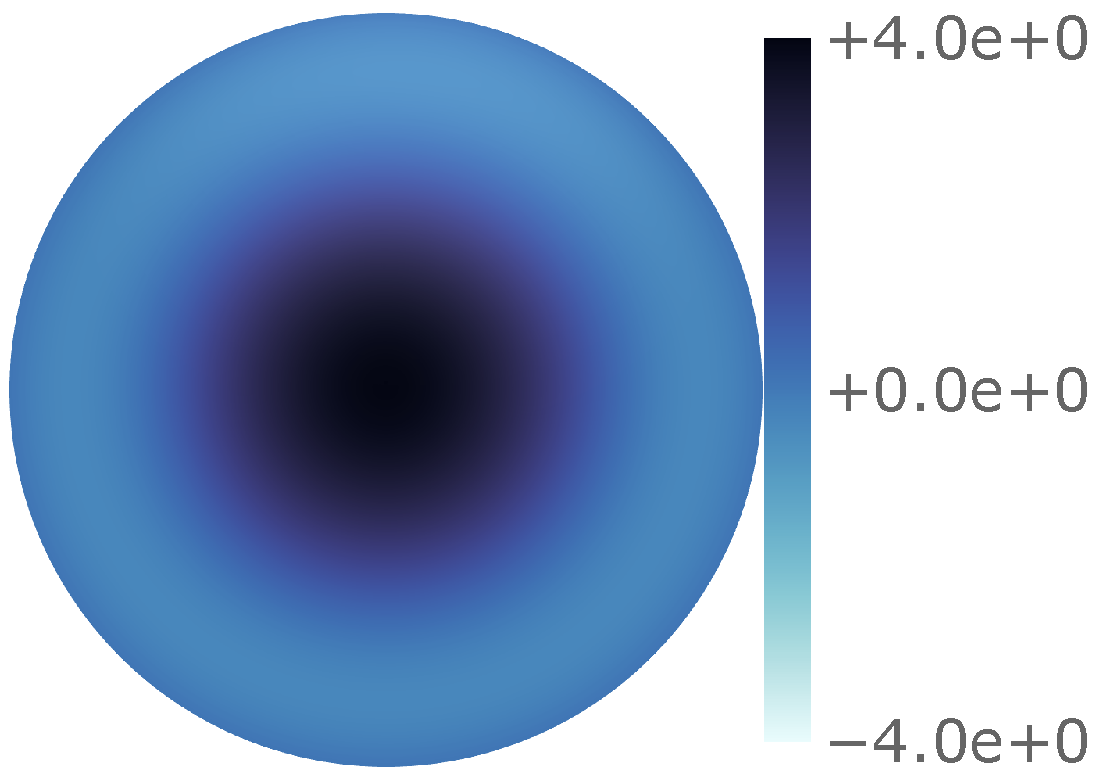
\includegraphics[trim={4 7 3 6},clip,width=.33\textwidth]{axisymmetric_wavelets_3B_2jmin_scaling_L128_res512_real.pdf}}
	\hfill
	\subfloat[\(\pixel{\Psi^{2j}}\)]
	{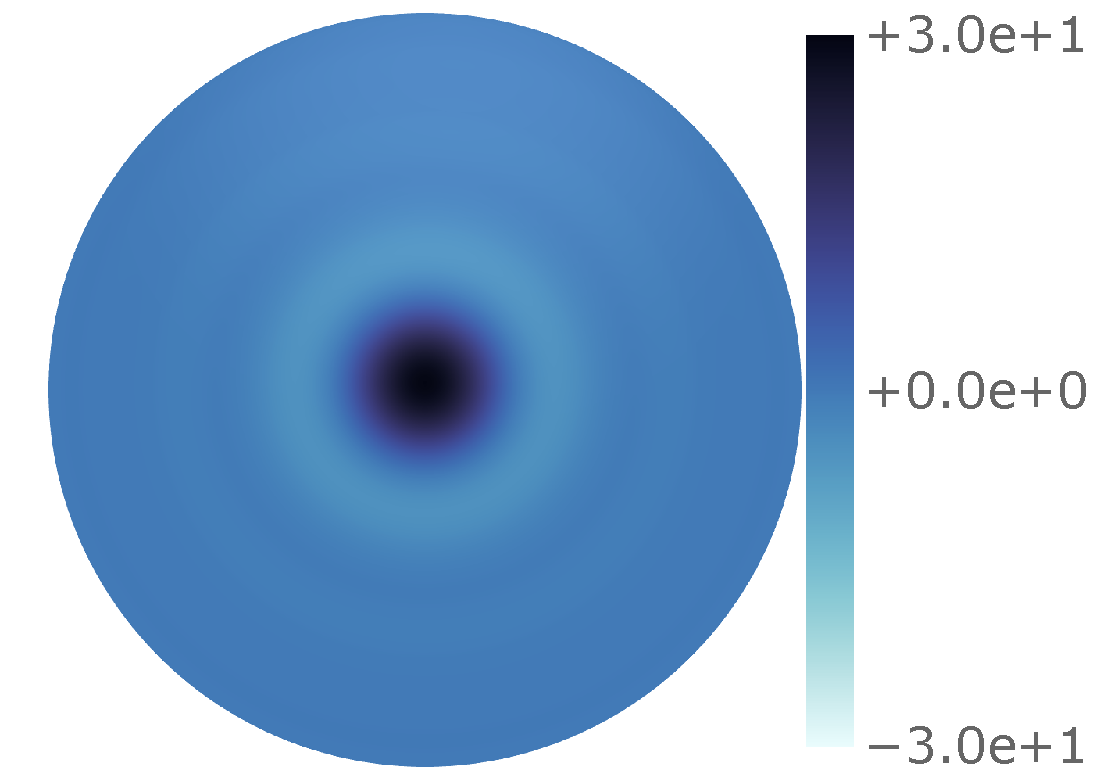
\includegraphics[trim={4 7 3 6},clip,width=.33\textwidth]{axisymmetric_wavelets_3B_2jmin_2j_L128_res512_real.pdf}}
	\hfill
	\subfloat[\(\pixel{\Psi^{3j}}\)]
	{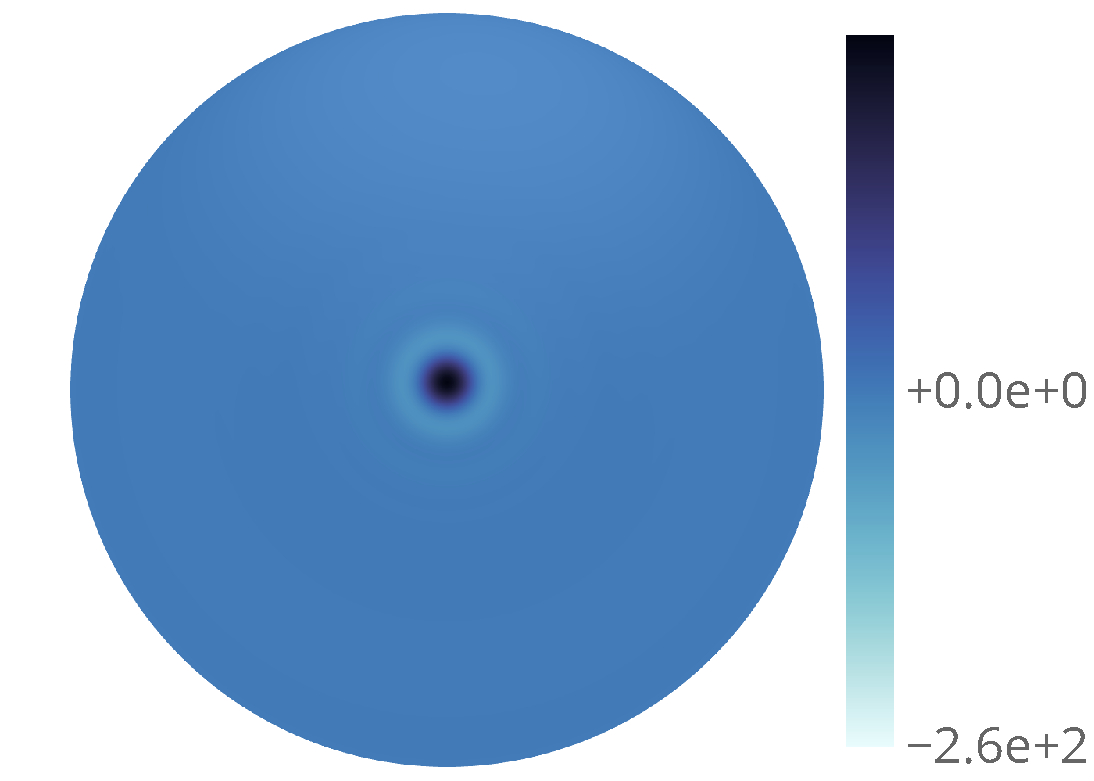
\includegraphics[trim={4 7 3 6},clip,width=.33\textwidth]{axisymmetric_wavelets_3B_2jmin_3j_L128_res512_real.pdf}}
	\newline
	\subfloat[\(\pixel{\Psi^{4j}}\)]
	{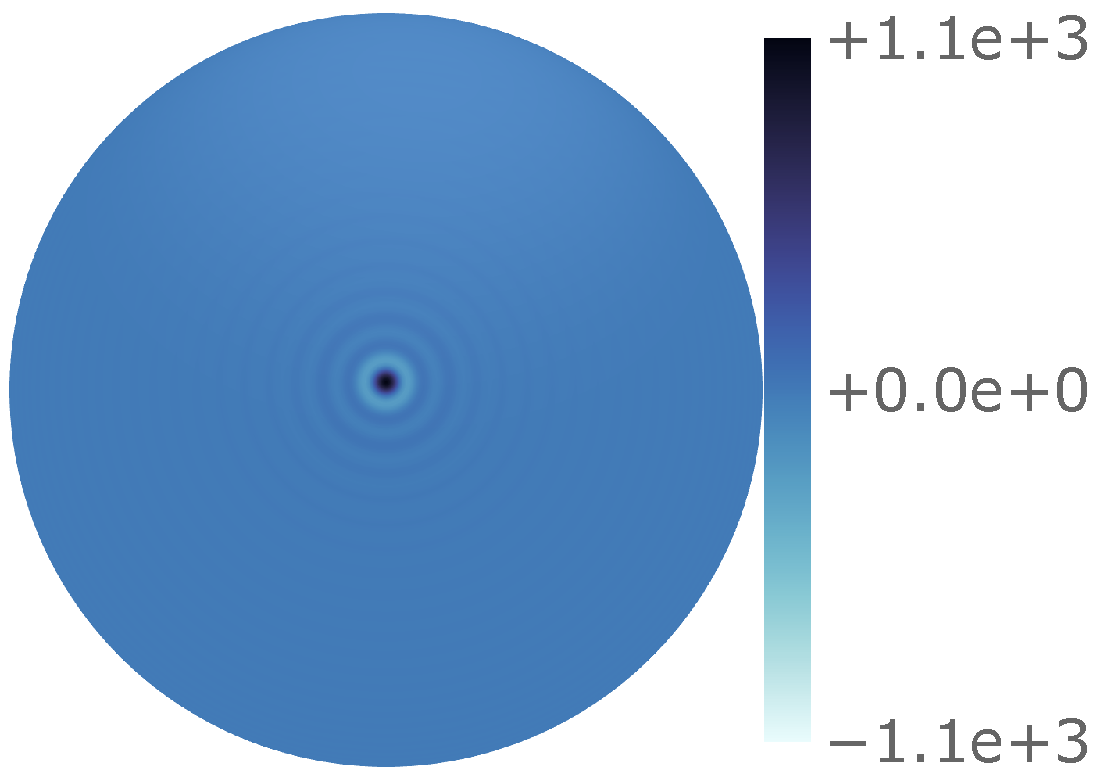
\includegraphics[trim={4 7 3 6},clip,width=.33\textwidth]{axisymmetric_wavelets_3B_2jmin_4j_L128_res512_real.pdf}}
	%
	\subfloat[\(\pixel{\Psi^{5j}}\)]
	{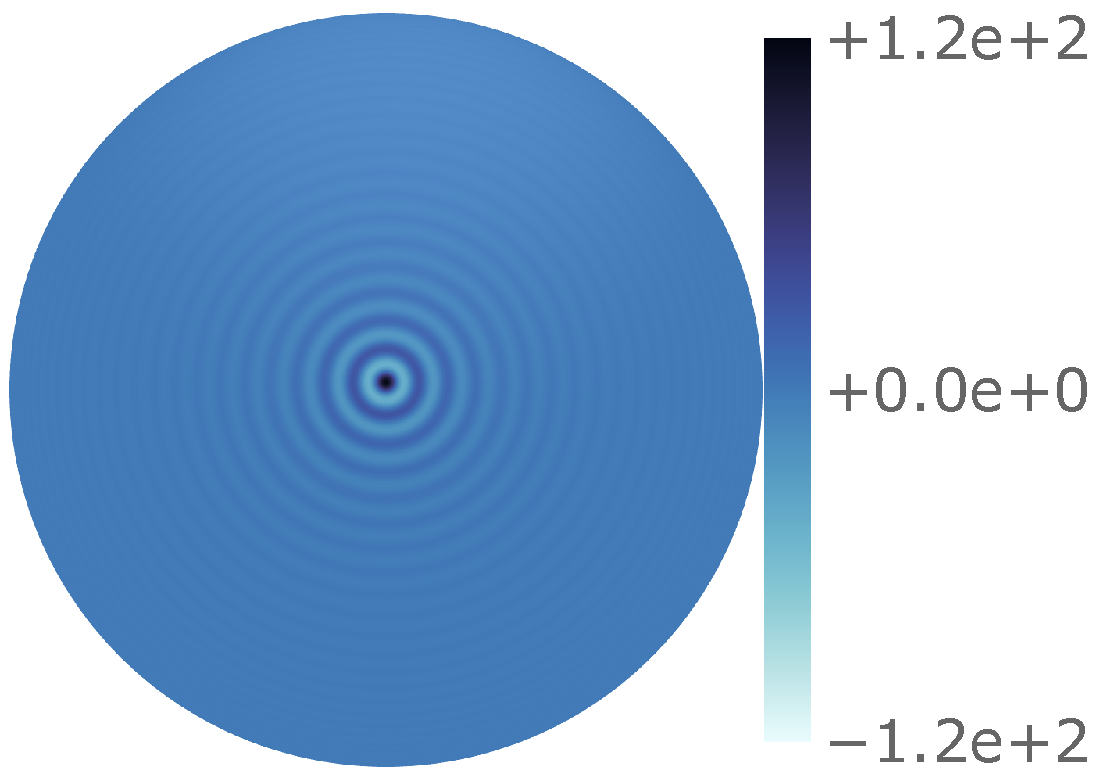
\includegraphics[trim={4 7 3 6},clip,width=.33\textwidth]{axisymmetric_wavelets_3B_2jmin_5j_L128_res512_real.pdf}}
	\caption[
		Some axisymmetric scale-discretised wavelets on the sphere
	]{
		The scaling function and the wavelets for scales \(j \in \set{2, 3, 4, 5}\) of the axisymmetric scale-discretised wavelets on the sphere centred on the north pole shown left-to-right, top-to-bottom.
		They are constructed through a tiling of the harmonic line with parameters \(\lambda=3\), \(J_{0}=2\), and bandlimit \(L=128\) (\cf{} \cref{fig:chapter2_tiling}).
	}\label{fig:chapter2_axisymmetric_wavelets}
\end{figure}


\section{Spectral Concentration Problem}

In the 1960s, Slepian, Landau and Pollak solved the fundamental problem of optimally concentrating a signal simultaneously in time and frequency~\cite{Landau1961,Landau1962,Slepian1983,Slepian1961}.
The resulting orthogonal family of functions, and their discrete and multidimensional counterparts~\cite{Bronez1988,Hanssen1997,Liu1992,Slepian1964,Slepian1978}, form the basis of a range of spectral analyses (\eg{}~\cite{Thomson1982,Thomson1990}).
\cref{sec:chapter2_slepian_euclidean} follows with a brief review of the initial time-frequency concentration problem, this is then proceeded with the extension to the spherical domain in \cref{sec:chapter2_slepian_sphere}.

\subsection{Euclidean: Time-Frequency Domain}\label{sec:chapter2_slepian_euclidean}

Before considering the Slepian spatial-spectral concentration problem in the spherical domain, first consider the one-dimensional, continuous-continuous, time-frequency concentration problem.
Here, a normalisation convention is adopted such that a real-valued time-domain single \(f(t)\) and its Fourier transform \(F(\varpi)\) are related by
%
\begin{equation}
	f(t)
	%
	= \frac{1}{2\pi} \int\limits_{\infty}^{\infty} \dd{\varpi} F(\varpi) \exp(i\varpi t)
\end{equation}
%
and
%
\begin{equation}
	F(\varpi)
	%
	= \int\limits_{\infty}^{\infty} \dd{\varpi} f(t) \exp(-i\varpi t),
\end{equation}
%
where \(t\) and \(\varpi{}\) denote the time and angular frequency respectively.
Slepian and Pollak~\cite{Slepian1961} considered the problem of optimally concentrating a strictly bandlimited signal \(f(t)\), with a spectrum \(F(\varpi)\) which disappears into a time interval \(\abs{t} \leq T\) for frequencies \(\abs{\varpi} < W\).
Through the \emph{Paley-Wiener} theorem, no bandlimited signal \(g(t)\) can be exactly concentrated within a finite interval~\cite{Daubechies1992,Mallat2008}.
To find the optimally concentrated signal, one must maximise the following ratio:
%
\begin{equation}\label{eq:chapter2_frequency_ratio}
	\mu
	%
	= \frac{\displaystyle\int\limits_{-T}^{T} \dd{t} \abs{g(t)}^{2}}
	%
	{\displaystyle\int\limits_{-\infty}^{\infty} \dd{t} \abs{g(t)}^{2}},
\end{equation}
%
although other criteria have been considered~\cite{Freeden1997,Riedel1995}.
Bandlimited signals \(g(t)\) which satisfy \cref{eq:chapter2_frequency_ratio}, have spectra \(G(\varpi)\) which satisfy the convolutional integral eigenproblem in the frequency-domain
%
\begin{equation}\label{eq:chapter2_frequency_eigenproblem}
	\int\limits_{-W}^{W} \dd{\varpi'} \frac{\sin{T(\varpi-\varpi')}}{\pi(\varpi-\varpi')} G(\varpi')
	%
	= \mu G(\varpi),
\end{equation}
%
where \(\abs{\varpi} \leq W\).

Slepian also considered the similar case of concentrating the spectrum \(H(\varpi)\) of a strictly timelimited function \(h(t)\), which disappears into a spectral interval \(\abs{\varpi} \leq W\) for times \(\abs{t} < T\).
The ratio to maximise here is
%
\begin{equation}\label{eq:chapter2_time_ratio}
	\mu
	%
	= \frac{\displaystyle\int\limits_{-W}^{W} \dd{\varpi} \abs{H(\varpi)}^{2}}
	%
	{\displaystyle\int\limits_{-\infty}^{\infty} \dd{\varpi} \abs{H(\varpi)}^{2}},
\end{equation}
%
which results in the time-domain eigenproblem
%
\begin{equation}\label{eq:chapter2_time_eigenproblem}
	\int\limits_{-T}^{T} \dd{t'} \frac{\sin{W(t-t')}}{\pi(t-t')} h(t')
	%
	= \mu h(t),
\end{equation}
%
where \(\abs{t} < T\).
In either case, the eigenvalues (which represent effective concentration) satisfy
%
\begin{equation}
	1 > \mu_{1} \geq \mu_{2} \geq \ldots > 0, % chktex 11
\end{equation}
%
with associated eigenfunctions, \eg{}
%
\begin{equation}
	g_{1}(t),\ g_{2}(t),\ \ldots
\end{equation}
%
which exist in the interval \(\abs{t} \leq T\).
Through a change of variables, the ratios \cref{eq:chapter2_frequency_ratio,eq:chapter2_time_ratio} may be transformed into one dimensionless eigenproblem:
%
\begin{equation}
	\int\limits_{-1}^{1} \dd{x'} \frac{\sin{TW(x-x')}}{\pi(x-x')} \psi(x')
	%
	= \mu \psi(x),
\end{equation}
%
where \(\abs{x} \leq 1\).
Hence, the eigenvalues and scaled eigenfunctions only depend on the time-bandwith product \(TW\).
Consider the sum of the eigenvalues
%
\begin{equation}
	N
	%
	= \sum\limits_{\alpha=1}^{\infty} \mu_{\alpha}
	%
	= \frac{2TW}{\pi}.
\end{equation}
%
The so-called Shannon number~\cite{Percival1993} \(N\) introduced here is a good estimate of the number of significant eigenvalues, which arises due to the characteristic shape of the eigenvalue spectrum~\cite{Landau1965,Slepian1965}.
Equivalently, this can be viewed as the number of signals \(f(t)\) which can be well-concentrated both into a finite time interval \(\abs{t} \leq T\) and a finite frequency interval \(\abs{\varpi} \leq W\).
Many of the results discussed above have analogues in the spatial-spectral concentration problem on the sphere, which is elaborated in \cref{sec:chapter2_slepian_sphere}.

\subsection{Sphere: Spatial-Spectral Domain}\label{sec:chapter2_slepian_sphere}

The two sub-spaces of interest of all square-integrable functions on the sphere \(\twoSphere{}\) are: \(\spaceSpacelimit{}\) the space of all spacelimited functions strictly contained within a region \(R\), and \(\spaceBandlimit{}\) the space of all bandlimited functions with no power above the bandlimit \(L\).
Similar to the Euclidean setting, no function can be strictly spacelimited as well as strictly bandlimited, \ie{} no \(\pixel{f}\) can be in both sub-spaces \(\spaceSpacelimit{}\) and \(\spaceBandlimit{}\) at the same time.
Thus, one may find either: the spacelimited functions \(\pixel{h} \in \spaceSpacelimit{}\) whose spectrum is optimally concentrated within the interval \(0 \leq \ell < L\), or the bandlimited functions \(\pixel{g} \in \spaceBandlimit{}\) which are optimally concentrated within a region \(R\).

\subsubsection{Spectral Concentration of a Spacelimited Function}

To maximise the concentration of a spacelimited function \(\pixel{h} \in \spaceSpacelimit{}\) within an interval \(0 \leq \ell < L\) one must maximise the ratio:
%
\begin{equation}\label{eq:chapter2_spacelimited_ratio}
	\mu
	%
	= \frac{\displaystyle\sum\limits_{\ell=0}^{L-1} \sum\limits_{m=-\ell}^{\ell} \abs{\harmonic{h}}^{2}}
	%
	{\displaystyle\sum\limits_{\ell=0}^{\infty} \sum\limits_{m=-\ell}^{\ell} \abs{\harmonic{h}}^{2}},
\end{equation}
%
which is analogous to the one-dimensional problem \cref{eq:chapter2_time_ratio}.
By substituting the expansion of the spherical harmonic coefficients
%
\begin{equation}
	\harmonic{h}
	%
	= \integrateRegion{\sphereVolume} \pixel{h} \pixel{\conj{\harmonic{Y}}},
\end{equation}
%
and swapping the order of summation and integration, the variational problem \cref{eq:chapter2_spacelimited_ratio} becomes
%
\begin{equation}
	\mu
	%
	= \frac{\integrateRegion{\sphereVolume[']} \pixel[']{h} \integrateRegion{\sphereVolume} \pixel{\delta_{\omega'}} \pixel{\conj{h}}}
	%
	{\integrateRegion{\sphereVolume} \abs{\pixel{h}}^{2}},
\end{equation}
%
where
%
\begin{equation}
	\pixel{\delta_{\omega'}}
	%
	= \sum\limits_{\ell=0}^{L-1} \sum\limits_{m=-\ell}^{\ell} \pixel[']{\conj{\harmonic{Y}}} \pixel{\harmonic{Y}}
\end{equation}
%
is the bandlimited Dirac delta function.
The maximally spacelimited functions \(\pixel{h} \in \spaceSpacelimit{}\) are therefore the solutions to the integral equation
%
\begin{equation}
	\integrateRegion{\sphereVolume} \pixel{\delta_{\omega'}} \pixel{\conj{h}}
	%
	= \mu \pixel[']{\conj{h}},
\end{equation}
%
which is the spherical equivalent of the one-dimensional time-domain eigenproblem \cref{eq:chapter2_time_eigenproblem}.

\subsubsection{Spatial Concentration of a Bandlimited Function}

Alternatively, to find the maximally concentrated bandlimited functions \(\pixel{g} \in \spaceBandlimit{}\) within a region \(R\) one must maximise the ratio:
%
\begin{equation}\label{eq:chapter2_bandlimited_ratio}
	\mu
	%
	= \frac{\integrateRegion{\sphereVolume} \abs{\pixel{g}}^{2}}{\integrateSphere{\omega} \abs{\pixel{g}}^{2}}
\end{equation}
%
which is, as before, analogous to the one-dimensional problem \cref{eq:chapter2_frequency_ratio}.
Expanding in harmonic space, and swapping the order of summation and integration, \cref{eq:chapter2_bandlimited_ratio} becomes
%
\begin{equation}
	\mu
	%
	= \frac{\displaystyle\sum\limits_{\ell=0}^{L-1} \sum\limits_{m=-\ell}^{\ell} \harmonic{g}
		%
		\sum\limits_{\ell'=0}^{L-1} \sum\limits_{m'=-\ell'}^{\ell'} \Dmatrix \conj{\harmonic[']{g}}}
	%
	{\displaystyle\sum\limits_{\ell=0}^{L-1} \sum\limits_{m=-\ell}^{\ell} \abs{\harmonic{g}}^{2}},
\end{equation}
%
where
%
\begin{equation}
	\Dmatrix
	%
	= \integrateRegion{\sphereVolume} \pixel{\harmonic{Y}} \pixel{\conj{\harmonic[']{Y}}}
\end{equation}
%
has been defined.
The eigenproblem, of which the maximally bandlimited functions arise from, is
%
\begin{equation}
	\sum\limits_{\ell'=0}^{L-1} \sum\limits_{m'=-\ell'}^{\ell'} \Dmatrix \conj{\harmonic[']{g}}
	%
	= \mu \conj{\harmonic{g}},
\end{equation}
%
which is analogous to the one-dimensional frequency-domain eigenproblem \cref{eq:chapter2_frequency_eigenproblem}.

\begin{figure}[htpb]
	\centering\capstart{}
	\subfloat[\(\mu_{1}=1.000000\)]
	{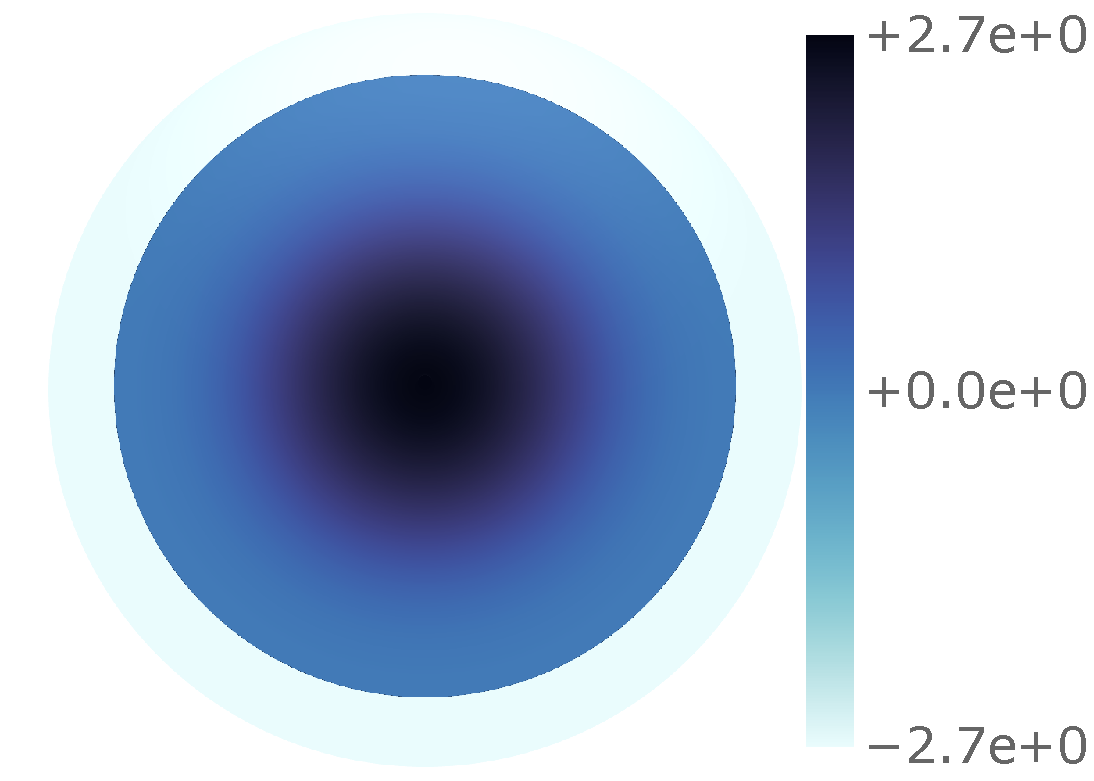
\includegraphics[trim={23 7 3 6},clip,width=.25\textwidth]{slepian_polar40_m0_rank0_lam1-000000e00_L16_res128_real.pdf}} % chktex 8
	\hfill
	\subfloat[\(\mu_{2}=0.999998\)]
	{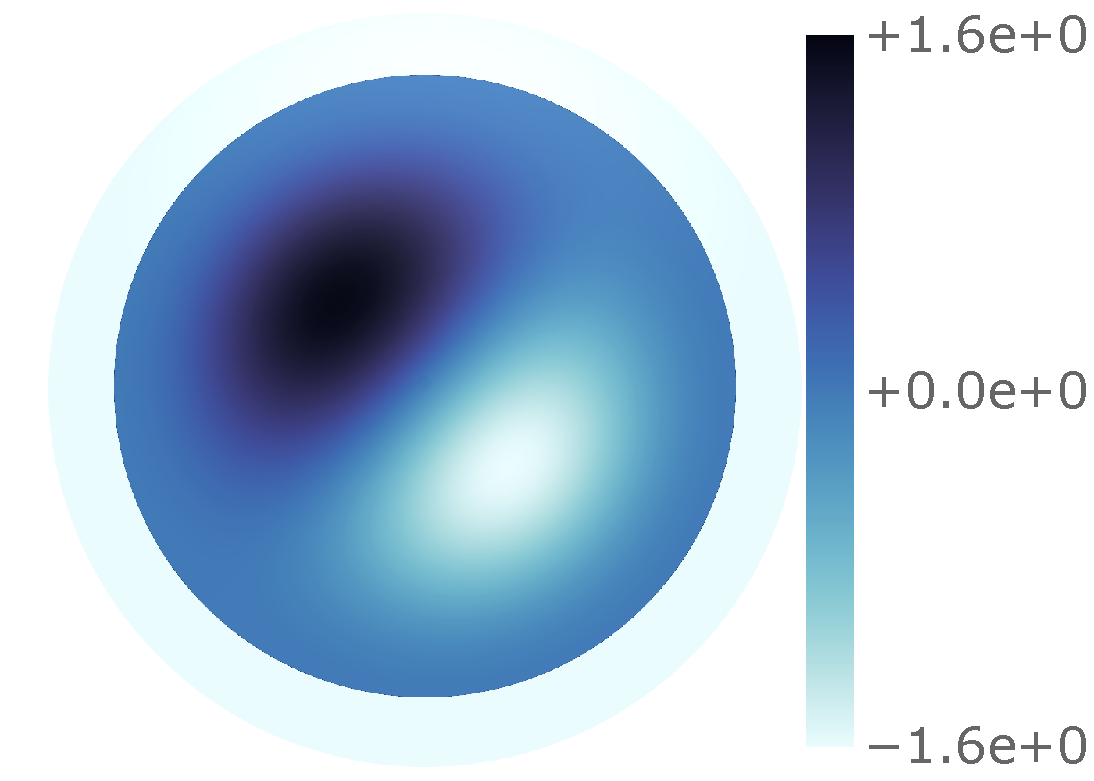
\includegraphics[trim={23 7 3 6},clip,width=.25\textwidth]{slepian_polar40_m-1_rank1_lam9-999984e-01_L16_res128_real.pdf}} % chktex 8
	\hfill
	\subfloat[\(\mu_{3}=0.999998\)]
	{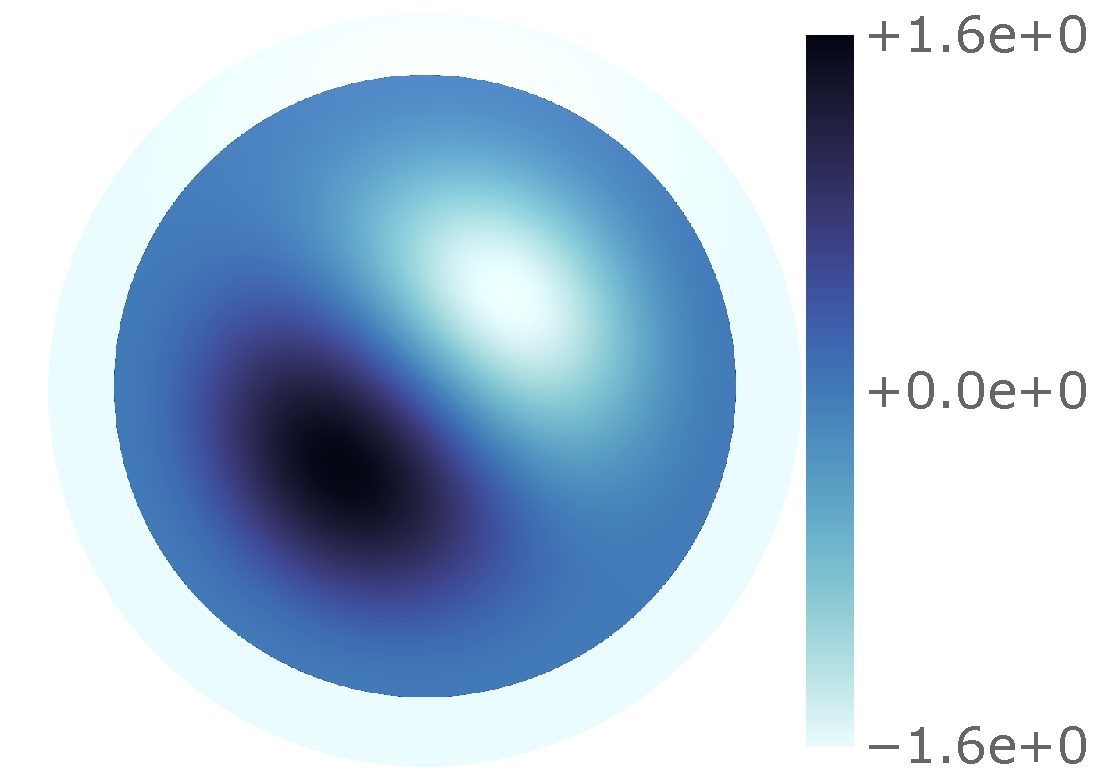
\includegraphics[trim={23 7 3 6},clip,width=.25\textwidth]{slepian_polar40_m1_rank2_lam9-999984e-01_L16_res128_real.pdf}} % chktex 8
	\hfill
	\subfloat[\(\mu_{4}=0.999966\)]
	{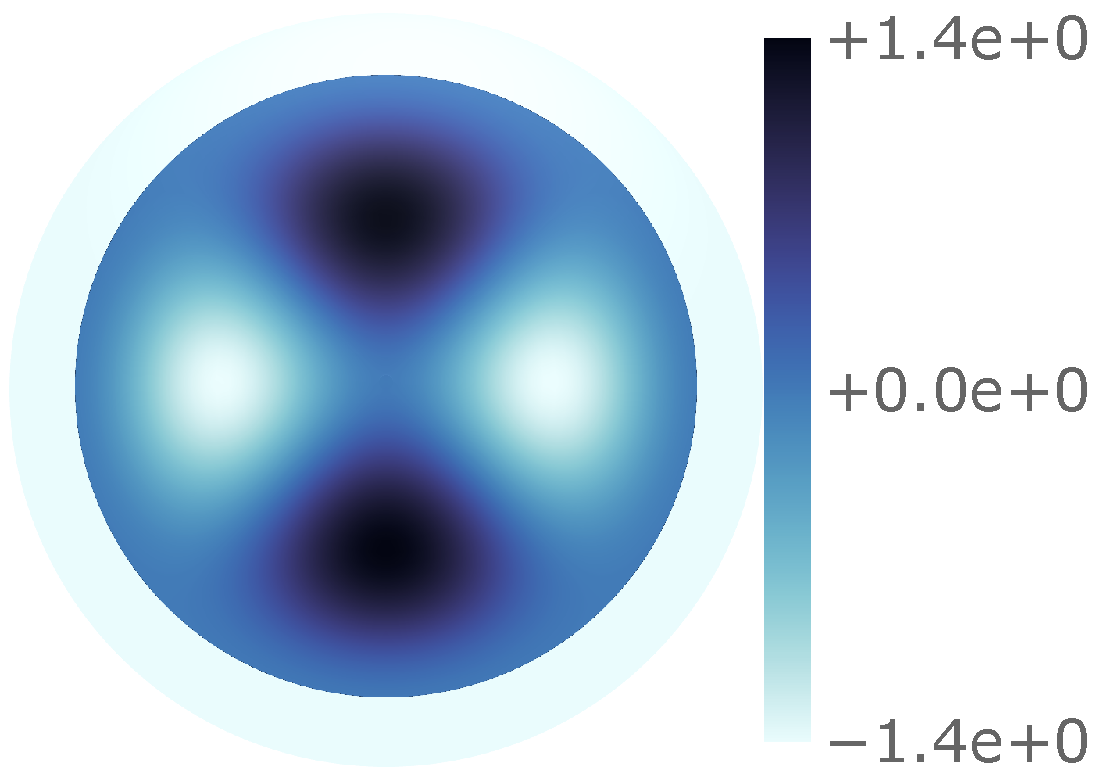
\includegraphics[trim={23 7 3 6},clip,width=.25\textwidth]{slepian_polar40_m-2_rank3_lam9-999664e-01_L16_res128_real.pdf}} % chktex 8
	\newline
	\subfloat[\(\mu_{5}=0.999966\)]
	{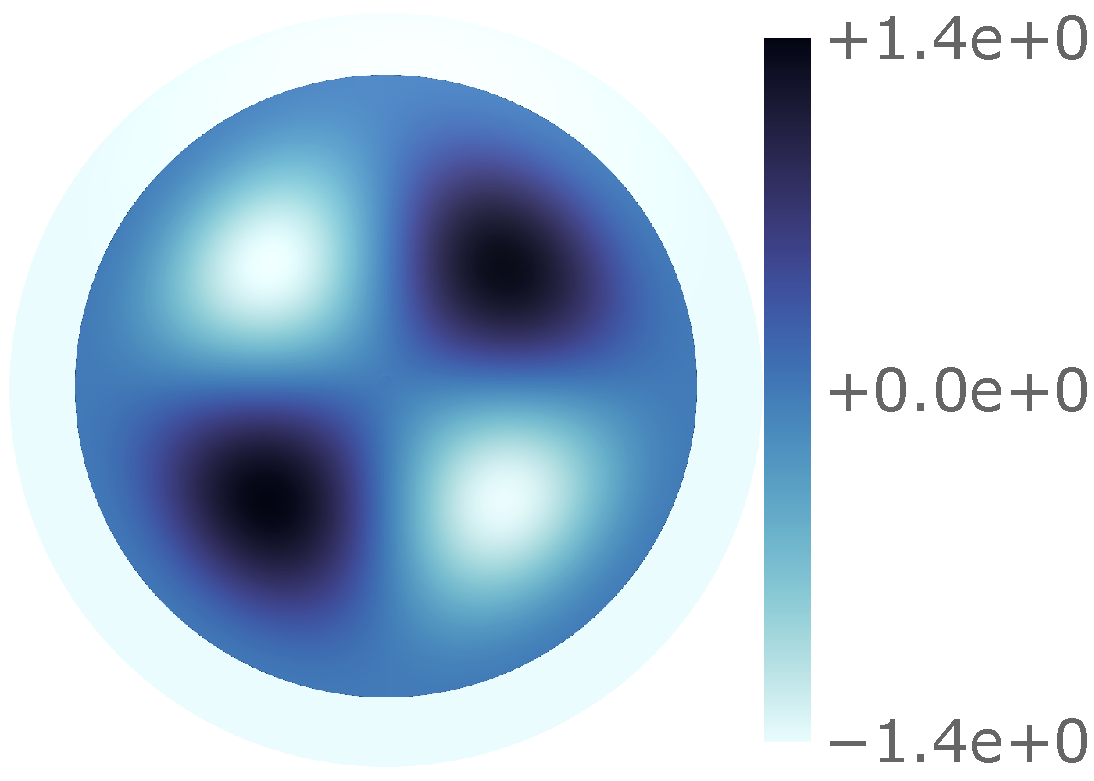
\includegraphics[trim={23 7 3 6},clip,width=.25\textwidth]{slepian_polar40_m2_rank4_lam9-999664e-01_L16_res128_real.pdf}} % chktex 8
	\hfill
	\subfloat[\(\mu_{6}=0.999939\)]
	{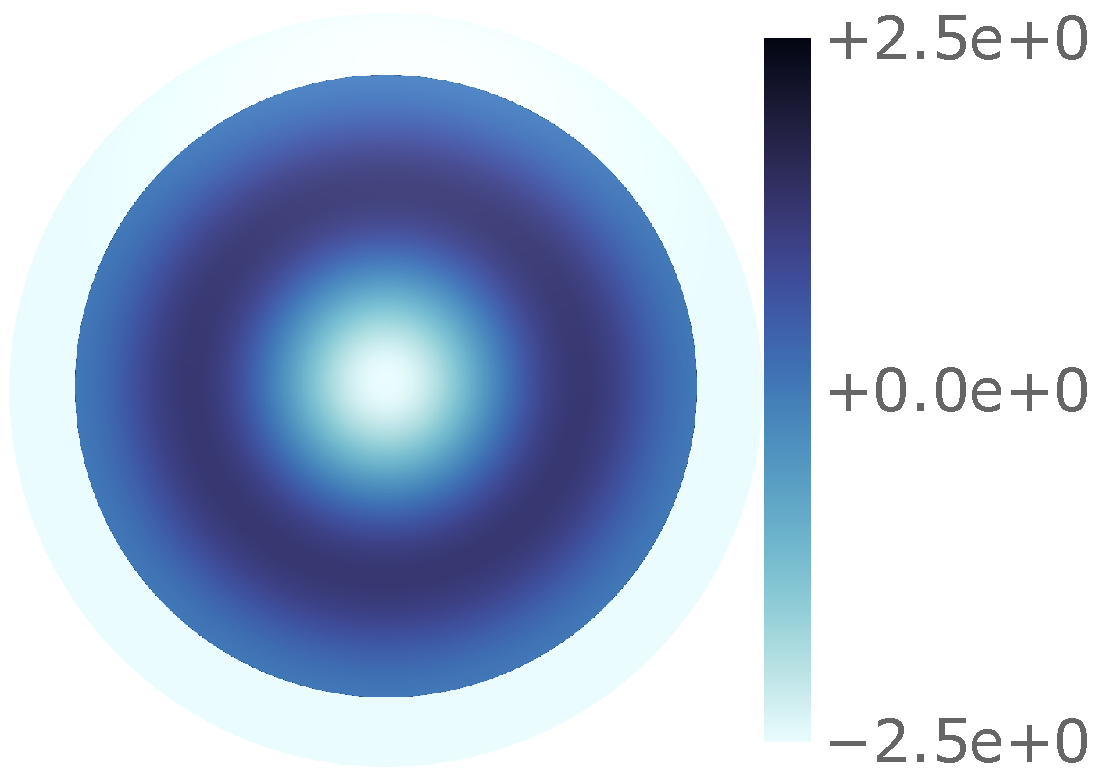
\includegraphics[trim={23 7 3 6},clip,width=.25\textwidth]{slepian_polar40_m0_rank5_lam9-999392e-01_L16_res128_real.pdf}} % chktex 8
	\hfill
	\subfloat[\(\mu_{7}=0.999553\)]
	{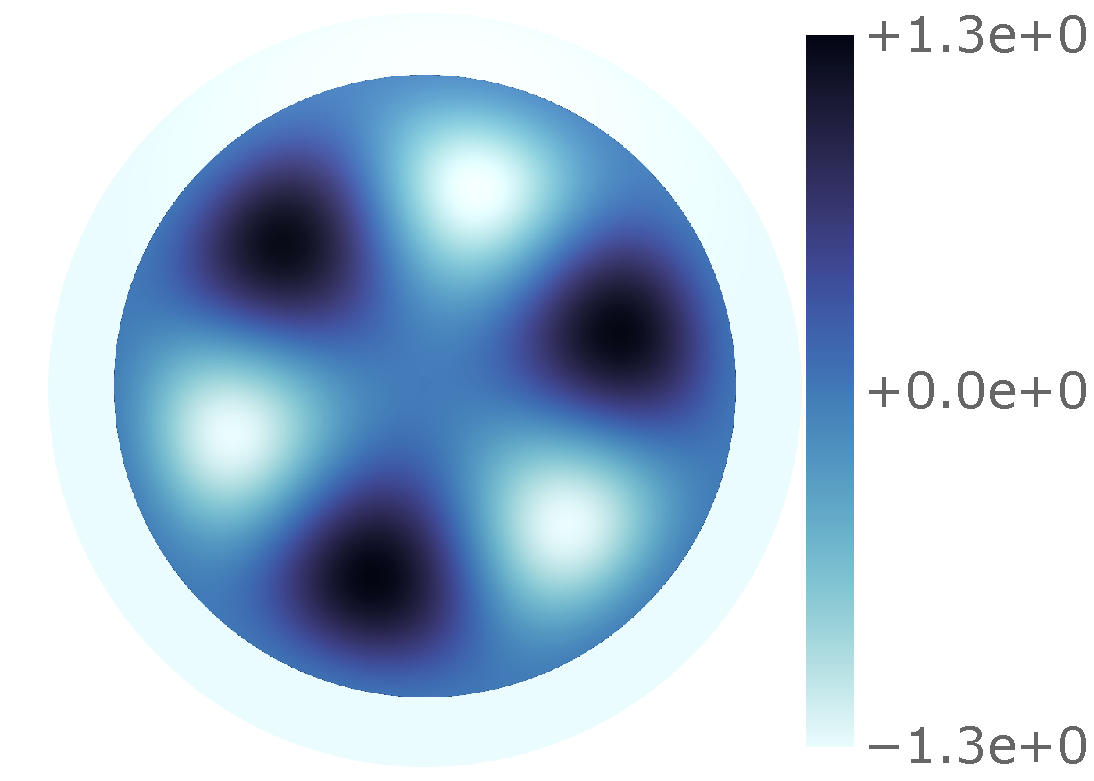
\includegraphics[trim={23 7 3 6},clip,width=.25\textwidth]{slepian_polar40_m-3_rank6_lam9-995528e-01_L16_res128_real.pdf}} % chktex 8
	\hfill
	\subfloat[\(\mu_{8}=0.999553\)]
	{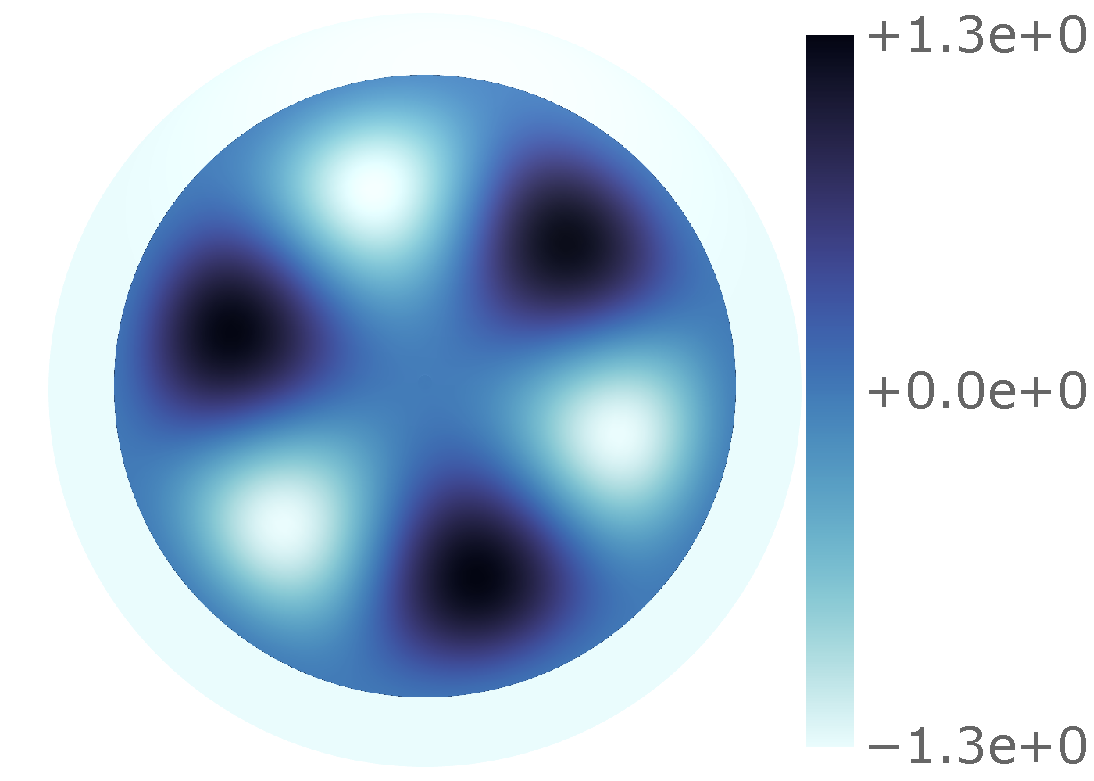
\includegraphics[trim={23 7 3 6},clip,width=.25\textwidth]{slepian_polar40_m3_rank7_lam9-995528e-01_L16_res128_real.pdf}} % chktex 8
	\newline
	\subfloat[\(\mu_{9}=0.998918\)]
	{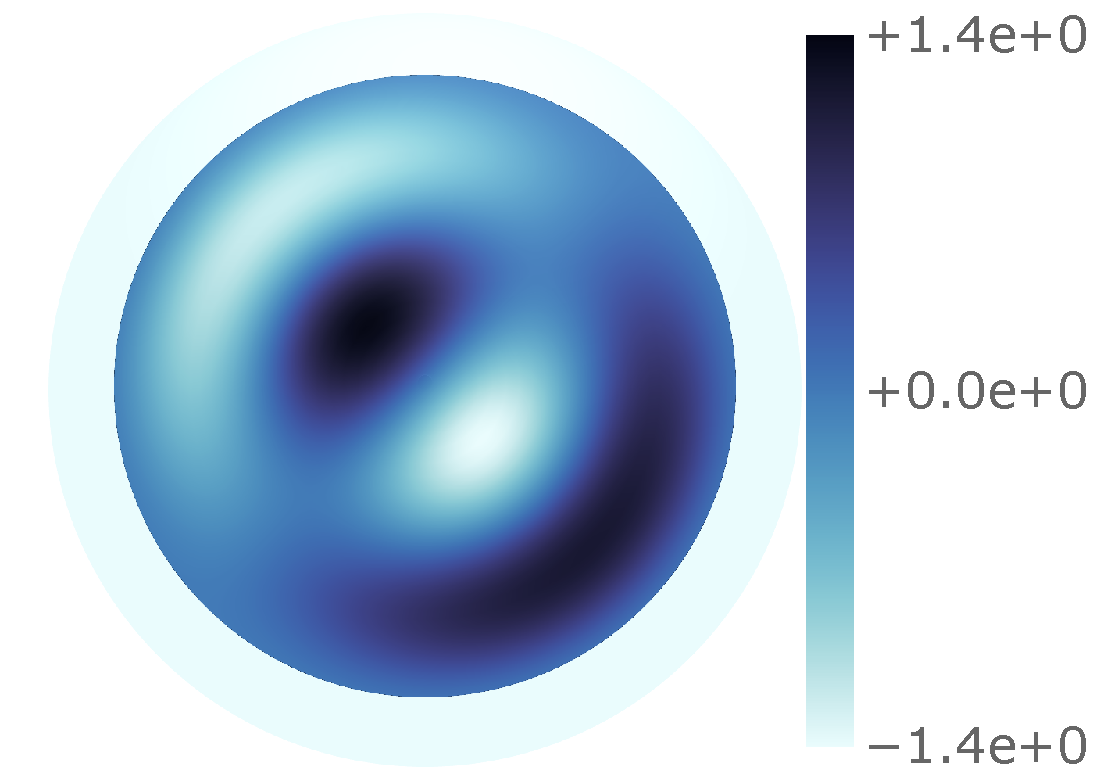
\includegraphics[trim={23 7 3 6},clip,width=.25\textwidth]{slepian_polar40_m-1_rank8_lam9-989180e-01_L16_res128_real.pdf}} % chktex 8
	\hfill
	\subfloat[\(\mu_{10}=0.998918\)]
	{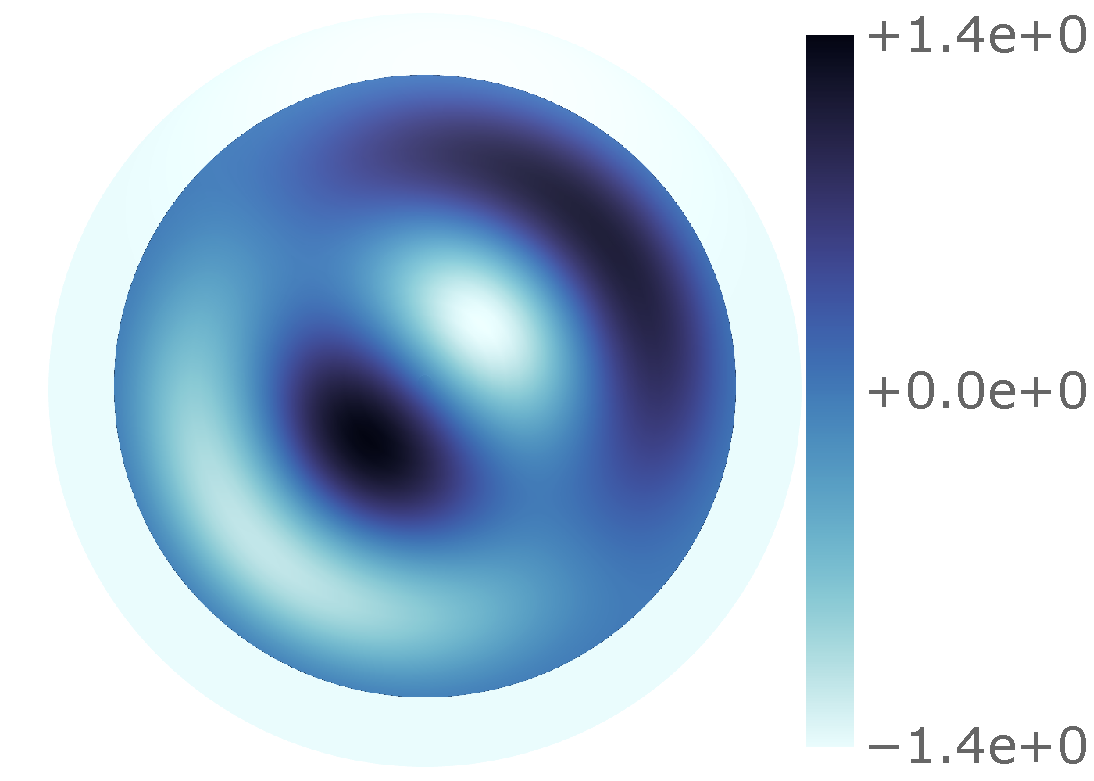
\includegraphics[trim={23 7 3 6},clip,width=.25\textwidth]{slepian_polar40_m1_rank9_lam9-989180e-01_L16_res128_real.pdf}} % chktex 8
	\hfill
	\subfloat[\(\mu_{11}=0.995897\)]
	{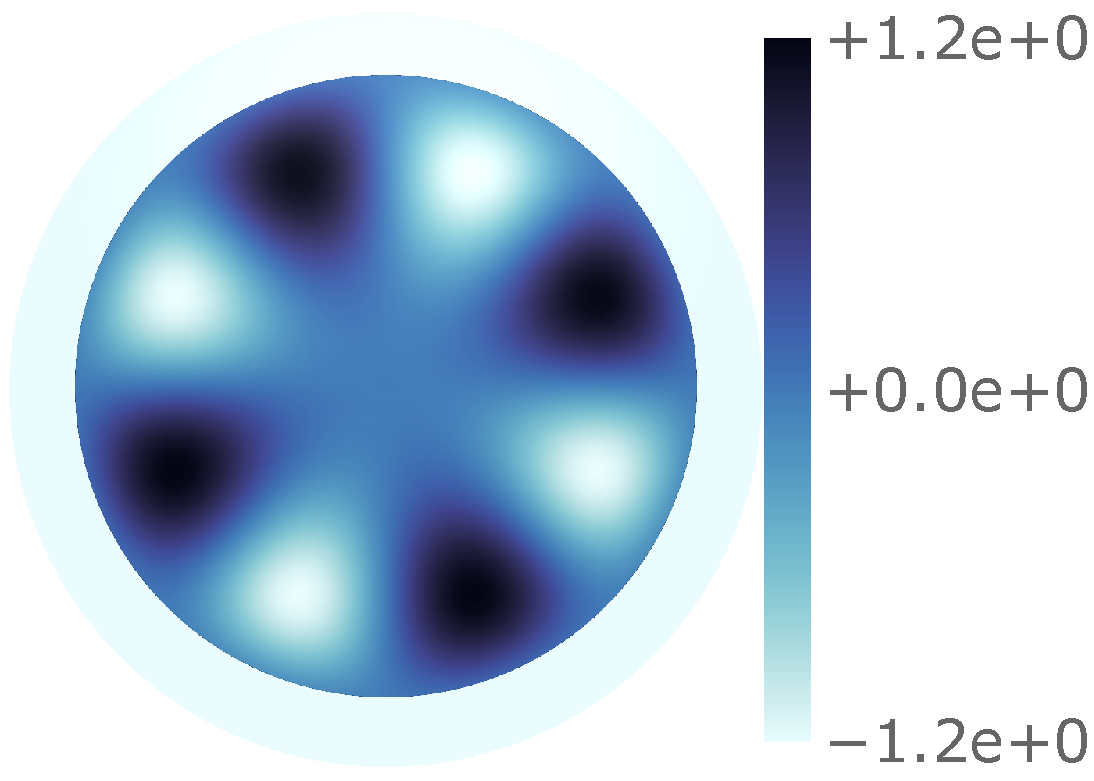
\includegraphics[trim={23 7 3 6},clip,width=.25\textwidth]{slepian_polar40_m-4_rank10_lam9-958971e-01_L16_res128_real.pdf}} % chktex 8
	\hfill
	\subfloat[\(\mu_{12}=0.995897\)]
	{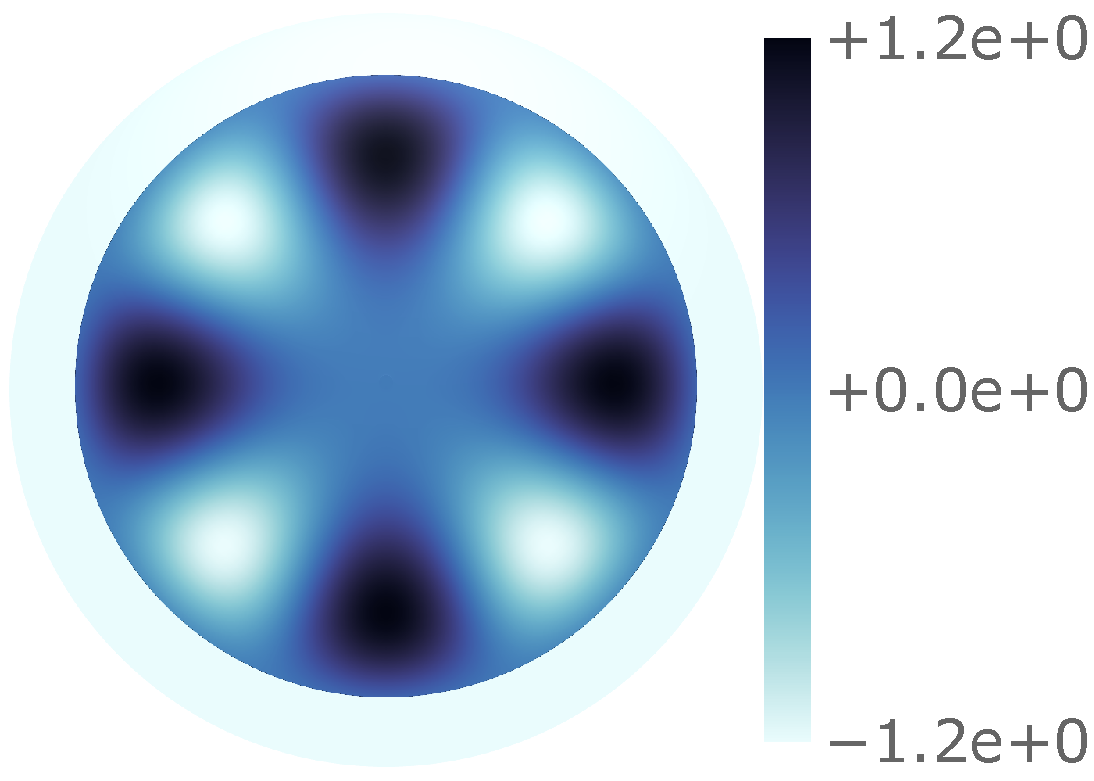
\includegraphics[trim={23 7 3 6},clip,width=.25\textwidth]{slepian_polar40_m4_rank11_lam9-958971e-01_L16_res128_real.pdf}} % chktex 8
	\newline
	\subfloat[\(\mu_{13}=0.988469\)]
	{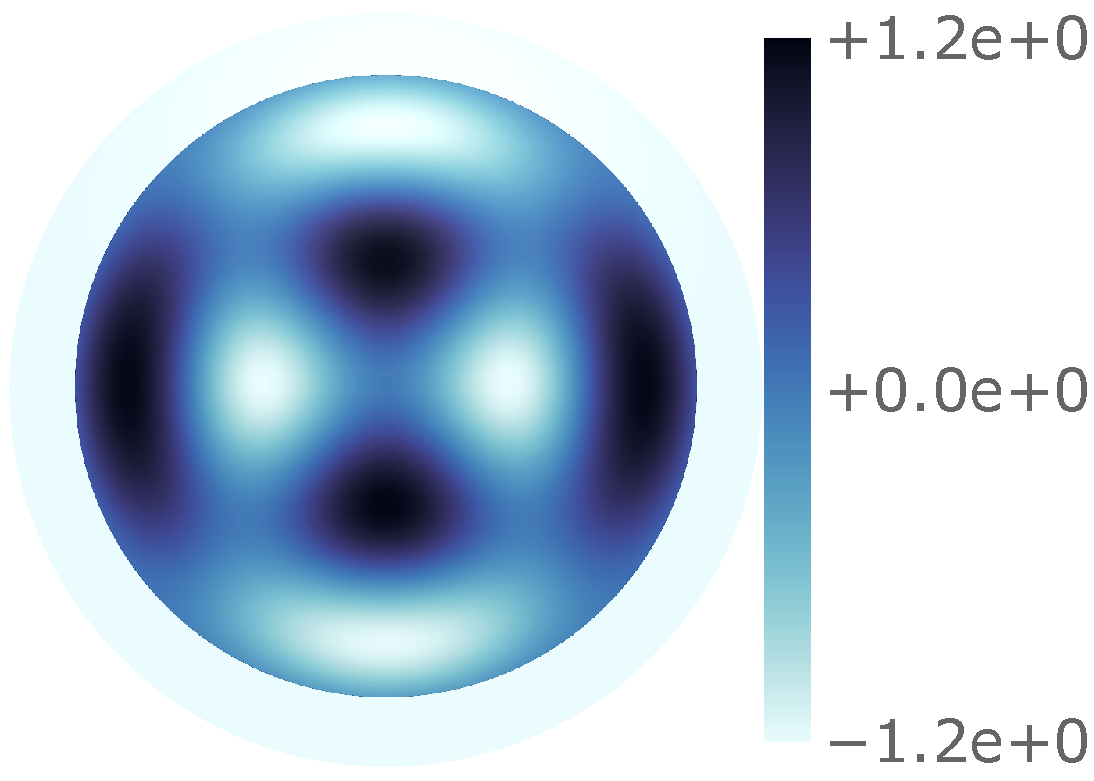
\includegraphics[trim={23 7 3 6},clip,width=.25\textwidth]{slepian_polar40_m-2_rank13_lam9-884688e-01_L16_res128_real.pdf}} % chktex 8
	\hfill
	\subfloat[\(\mu_{14}=0.988469\)]
	{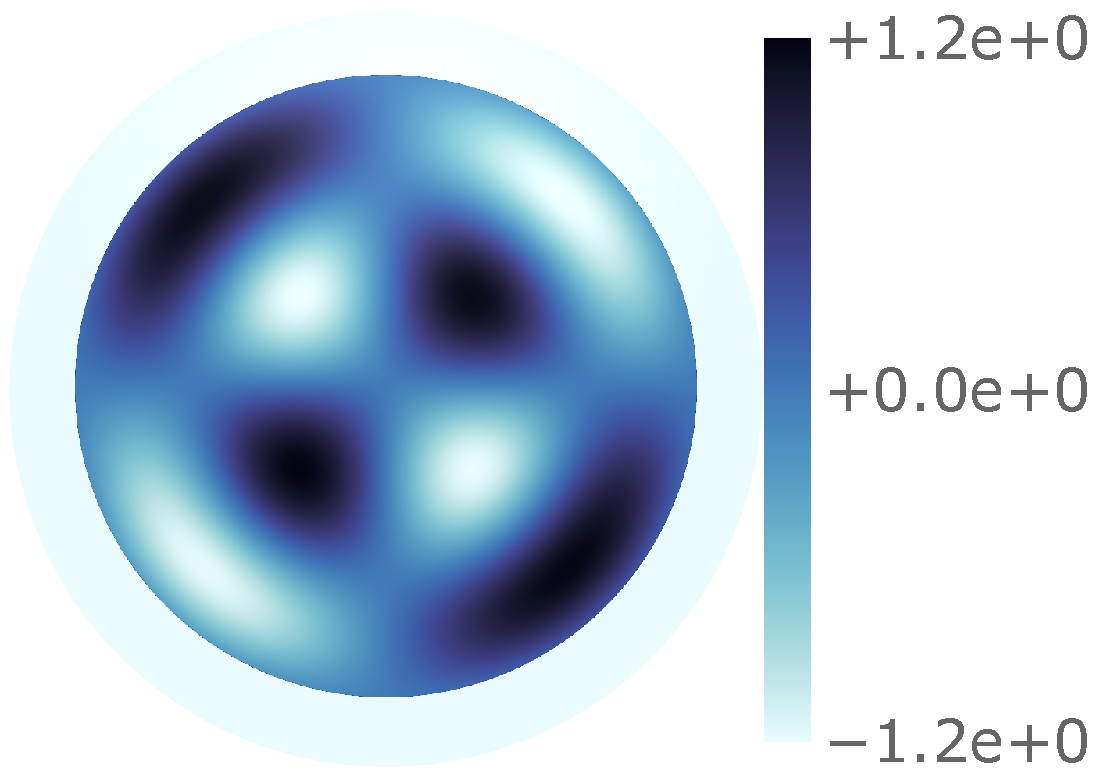
\includegraphics[trim={23 7 3 6},clip,width=.25\textwidth]{slepian_polar40_m2_rank12_lam9-884688e-01_L16_res128_real.pdf}} % chktex 8
	\hfill
	\subfloat[\(\mu_{15}=0.984654\)]
	{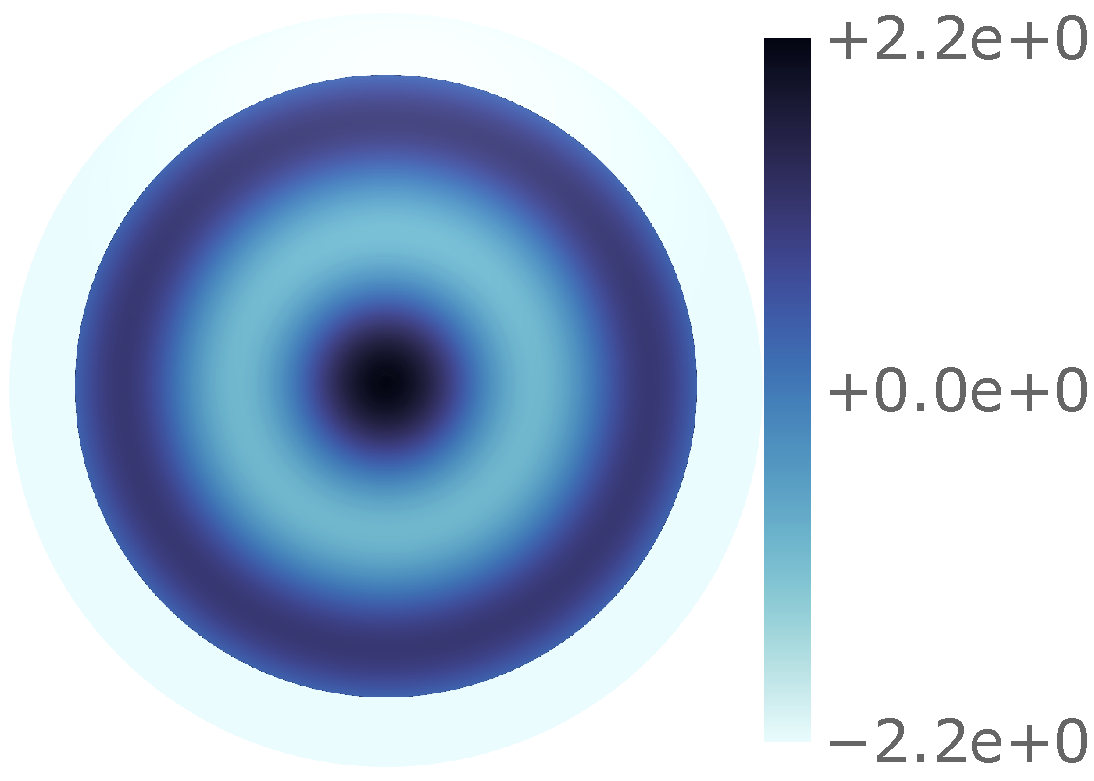
\includegraphics[trim={23 7 3 6},clip,width=.25\textwidth]{slepian_polar40_m0_rank14_lam9-846542e-01_L16_res128_real.pdf}} % chktex 8
	\hfill
	\subfloat[\(\mu_{16}=0.973439\)]
	{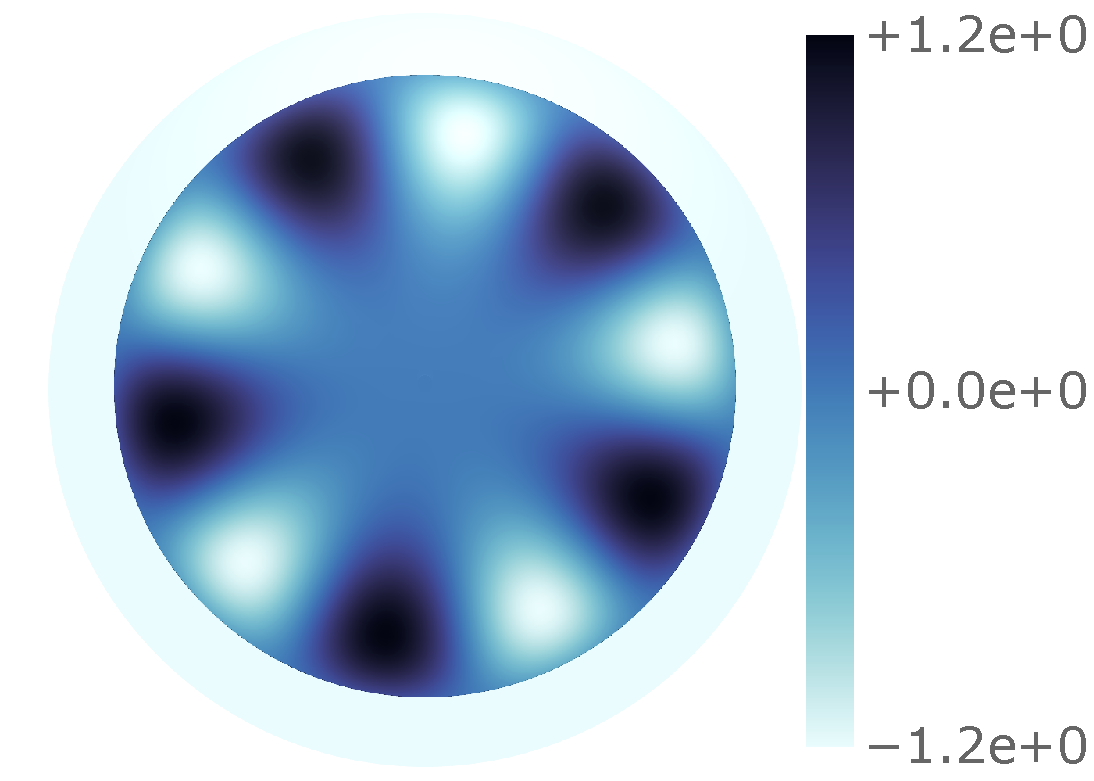
\includegraphics[trim={23 7 3 6},clip,width=.25\textwidth]{slepian_polar40_m5_rank15_lam9-734390e-01_L16_res128_real.pdf}} % chktex 8
	\caption[
		The Slepian functions within a \(\SI{40}{\degree}\) polar cap
	]{
		The first sixteen Slepian functions \(\pixel{\slepian{S}}\) within a polar cap of colatitudinal radius \(\Theta_{0}=\SI{40}{\degree}\).
		The bandlimit here is  \(L=16\), which corresponds to a Shannon number of \(N=30\).
		Ordered by decreasing eigenvalue, the plots are shown left-to-right, top-to-bottom --- indicating worse concentration within the region.
		Note the similarity with the spherical harmonics in this straightforward region.
	}\label{fig:chapter2_slepian_polar_cap}
\end{figure}


\begin{figure}[htpb]
	\centering\capstart{}
	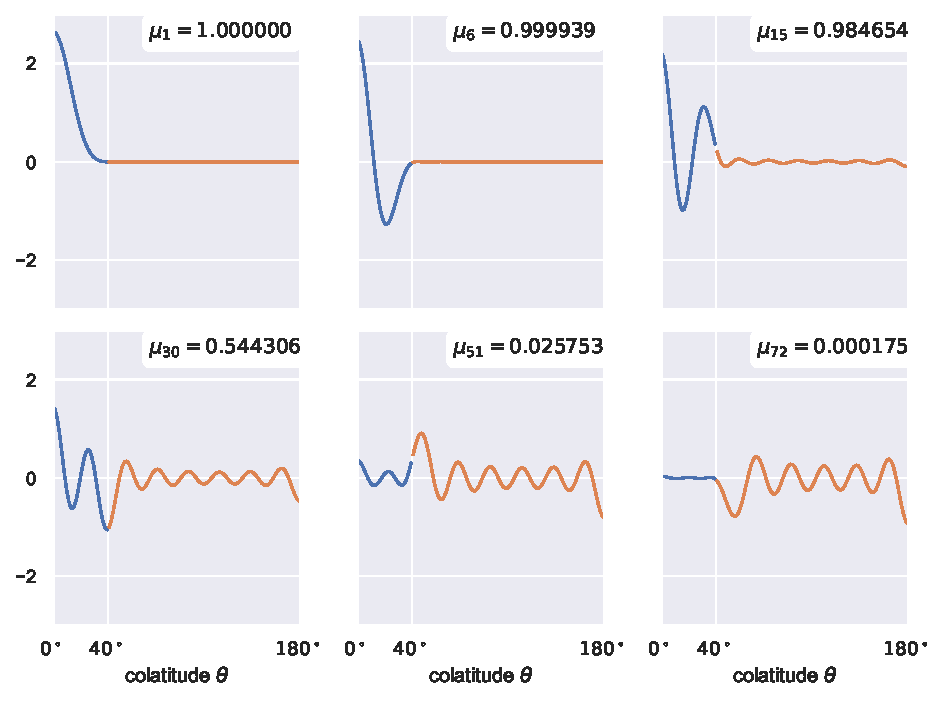
\includegraphics[width=\textwidth]{slepian_colatitude.pdf}
	\caption[
		The colatitudinal dependence of the polar cap Slepian functions
	]{
		The colatitudinal dependence of the Slepian functions \(\pixel{\slepian{S}}\) within a polar cap of colatitudinal radius \(\Theta_{0}=\SI{40}{\degree}\) for \(p \in \set{1, 6, 15, 30, 51, 72}\) shown left-to-right, top-to-bottom.
		The bandlimit here is  \(L=16\), which corresponds to a Shannon number of \(N=30\), \ie{} the final two panels are beyond the Shannon number.
		Blue curves show the concentration within the cap \(\SI{0}{\degree} \leq \theta \leq \Theta_{0}{}\), whilst orange curves show the leakage into the rest of the sphere \(\Theta_{0} < \theta \leq \SI{180}{\degree}\).
		The eigenvalue \(\mu{}\) quantifies the relative spatial concentration of the Slepian function, where lower values have increasing leakage into the orange curve.
	}\label{fig:chapter2_slepian_colatitude}
\end{figure}


\begin{figure}[htpb]
	\centering\capstart{}
	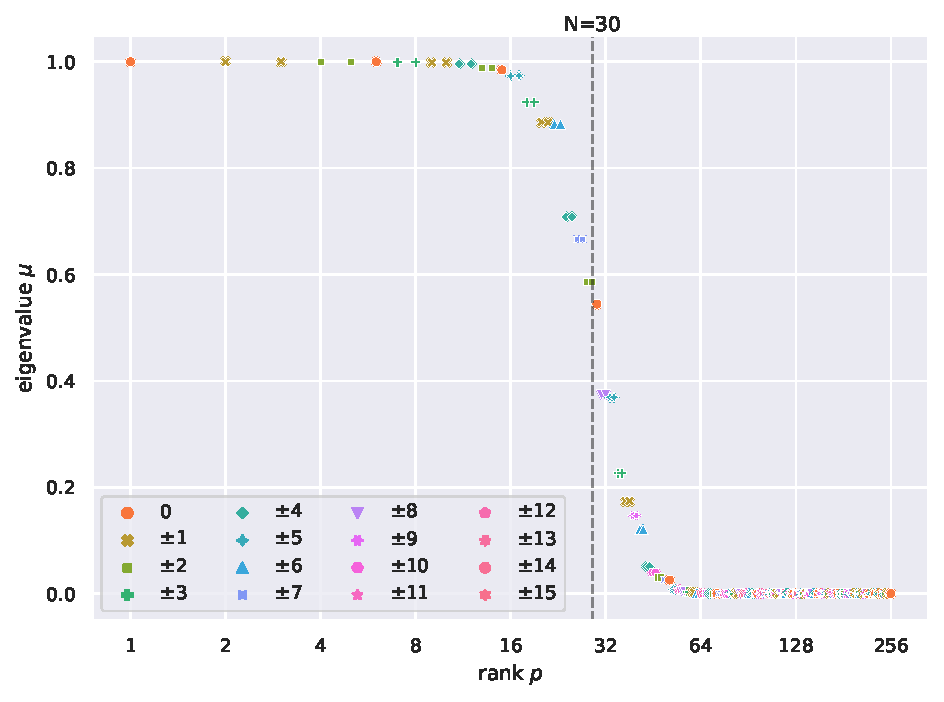
\includegraphics[width=\textwidth]{polar_cap_eigenvalues.pdf}
	\caption[
		The Slepian eigenvalues within a \(\SI{40}{\degree}\) polar cap
	]{
		The ordered Slepian eigenvalues within a polar cap of colatitudinal radius \(\theta_{0}=\SI{40}{\degree}\).
		The bandlimit here is \(L=16\), which corresponds to a Shannon number of \(N=30\), as indicated on the plot.
		Initially, the eigenvalues are \(\almost{1}\), before decreasing rapidly around the Shannon number, and where the majority of the later eigenvalues are \(\almost{0}\).
	}\label{fig:chapter2_polar_cap_eigenvalues}
\end{figure}


\section{Motivation}

\subsection{Overview}

\subsection{Cosmology}

\begin{figure}[htpb]
	\centering\capstart{}
	\includegraphics[trim={0 200 0 0},clip,width=\textwidth]{planck_2018_temp_freq.pdf}
	\includegraphics[trim={1100 0 1100 2100},clip,width=\textwidth]{planck_2018_temp_freq.pdf}
	\caption[
		The 2018 \emph{Planck} maps in intensity in each frequency band
	]{
		Fluctuations of sky emission in each of nine \emph{Planck} frequency bands, after removal of a common dipole component (courtesy of \emph{The Planck Collaboration 2018}~\cite{Planck2020}).
		Note that the CMB is obstructed by the foreground microwave emissions of the Milky Way at all frequencies.
	}\label{fig:chapter2_planck_frequency}
\end{figure}


\begin{figure}[htpb]
	\centering\capstart{}
	\includegraphics[width=\textwidth]{planck_2018_temp_mask.pdf}
	\caption[
		The 2018 \emph{Planck} CMB map extracted using the \texttt{SMICA} method
	]{
		The \texttt{SMICA}~\cite{Planck2020a} foreground-cleaned temperature map of the \emph{Planck} CMB sky (courtesy of \emph{The Planck Collaboration 2018}~\cite{Planck2020}).
		The CMB map has been masked, primarily around the Galactic plane (outlined in grey), and inpainted in regions where residuals from foreground emission are expected to be considerable.
		Slepian wavelets offer an alternative approach in which the wavelets are constructed in the region outside the mask.
	}\label{fig:chapter2_planck_unmasked}
\end{figure}


\subsection{Statistics of Random Fields on the Sphere}

\subsection{Observations Over the Partial Sphere}

\section{Outlook}

\subsection{Current Approaches}

\subsection{This Thesis}
